\documentclass[a4paper]{article}
\usepackage{hyperref}
\usepackage{graphicx}

\setlength{\oddsidemargin}{0in}
\setlength{\evensidemargin}{0in}
\setlength{\textwidth}{\paperwidth}
\addtolength{\textwidth}{-2in}
\setlength{\topmargin}{0in}
\setlength{\headsep}{1em}
\setlength{\textheight}{\paperheight}
\addtolength{\textheight}{-2in}
\setlength{\footskip}{2em}
\addtolength{\textheight}{-\footskip}

\newcommand{\Sup}{\mathrm{supp}} % Support of a fuzzy set 

\newtheorem{definition}{Definition}
\newtheorem{theorem}{Theorem}
\newenvironment{proof}{\noindent{\bf Proof:}}{\hfill $\Box$\medskip}
\newcounter{ex}
\newenvironment{example}{\addtocounter{ex}1\paragraph{Example \arabic{ex}}}%
  {\hfill $\bigstar$\medskip}

\title{RDF Mining: Ideas for research}
\author{Andrea G. B. Tettamanzi \and Catherine Faron Zucker \and Fabien Gandon\\
  WIMMICS Team\\
  Universit\'e de Nice Sophia Antipolis -- Laboratoire I3S -- INRIA\\
  andrea.tettamanzi@unice.fr, faron@polytech.unice.fr, fabien.gandon@inria.fr}

\begin{document}
  \maketitle

\begin{abstract}
  This is a working document with ideas on a research work bringing together
  the semantic Web, possibility theory, and evolutionary algorithms.
  % At this stage, the first author is the sole responsible for any errors or omissions.
\end{abstract}

\begin{flushright}
  \textit{Hypothesen sind Netze, nur der wird fangen, der auswirft.}\\
--- Novalis
\end{flushright}

\section{Introduction}

The Semantic Web has come of age.
The first massive deployment of its concept is the Linking Open Data (LOD) initiative,
which covers but the data layer of the Semantic Web.
RDF is the data model of this basic layer.
As of today, billions of RDF triples are available on the Web. They can be queried
by means of a specialized query language, SPARQL, through a number of SPARQL endpoints.

Now that the LOD is reality, the next question is what to make out of it.
An obvious answer to this question is to extract knowledge from it \cite{AuerLehmann2010swj}.
LOD is often considered as a giant knowledge base, not just raw data.
Now that the LOD has reached the status of ``big RDF data,'' we want to analyze
it and extract ``smart data'' from it, i.e., learn knowledge from it.
RDF data may be regarded as an oriented, labeled multigraph.
Therefore, it would appear that general methods and techniques that have been devised
for mining graphs should be relevant to mining linked open data.
Graph mining is the field of data mining that deals with
``mining data that is represented as a graph''~\cite{CookHolder2006}.
Graph mining methods have been successfully applied to a variety of problems, where
knowledge has to be extracted from chemical graphs, bioinformatics data,
Web graphs, and social networks. The main techniques employed in graph mining
are frequent substructure mining, link analysis, graph kernels, and graph grammars.
As a matter of fact, as it will become clear in the next sections,
our work does not focus on the graph structure of the knowledge represented using
the RDF formalism, but on its semantics and on the logical axioms that best describe
that knowledge. The approach we propose should therefore be regarded as complementary
to the general graph mining methods and specific to one kind of graph, namely
a particular family of graph-based knowledge-representation formalisms.

Some preliminary work in this direction has been done, which will be briefly surveyed
in Section~\ref{sec:survey}.
Workshops dedicated to this endeavor have been launched, including
the International Workshop on Knowledge Discovery and Data Mining meets Linked Open Data
({Know@LOD}), whose first edition took place at the 9th Extended Semantic Web Conference in 2012,
with the aim of presenting recent work on statistical schema induction, mapping, and link mining,
the \href{http://keg.vse.cz/dmold2013/}{Data Mining on Linked Data Workshop} (DMoLD),
which was held in 2013 in Prague during the European Conference on Machine Learning
and Principles and Practice of Knowledge Discovery in Databases (ECML/PKDD 2013),
and the International Workshop on Consuming On-Lind Linked Data (COLD),
which had its \href{http://db.uwaterloo.ca/cold2013/}{fourth edition} in 2013,
colocated with the 12th International Semantic Web Conference (ISWC) in Sydney, Australia.

Virtually all the approaches to the automated construction of ontologies on the
basis of RDF facts are based on ideas taken from Inductive Logic Programming
(cf.\ Section~\ref{ILP}). However, as Popper rightly observed~\cite{Popper1935},
there is no such thing as an inductive logic. The approach we propose,
whose main components are illustrated in Figure~\ref{fig:synopsis}, is inspired by
Popper's critical rationalism: hypotheses are generated by a mechanism, namely
evolutionary algorithms, which lays outside of Logic; they are then tested using
a deductive process, just like scientific theories are. Possibility theory is used
to capture what Popper calls the ``truth content'' of the hypotheses.

\begin{figure}
  \begin{center}
    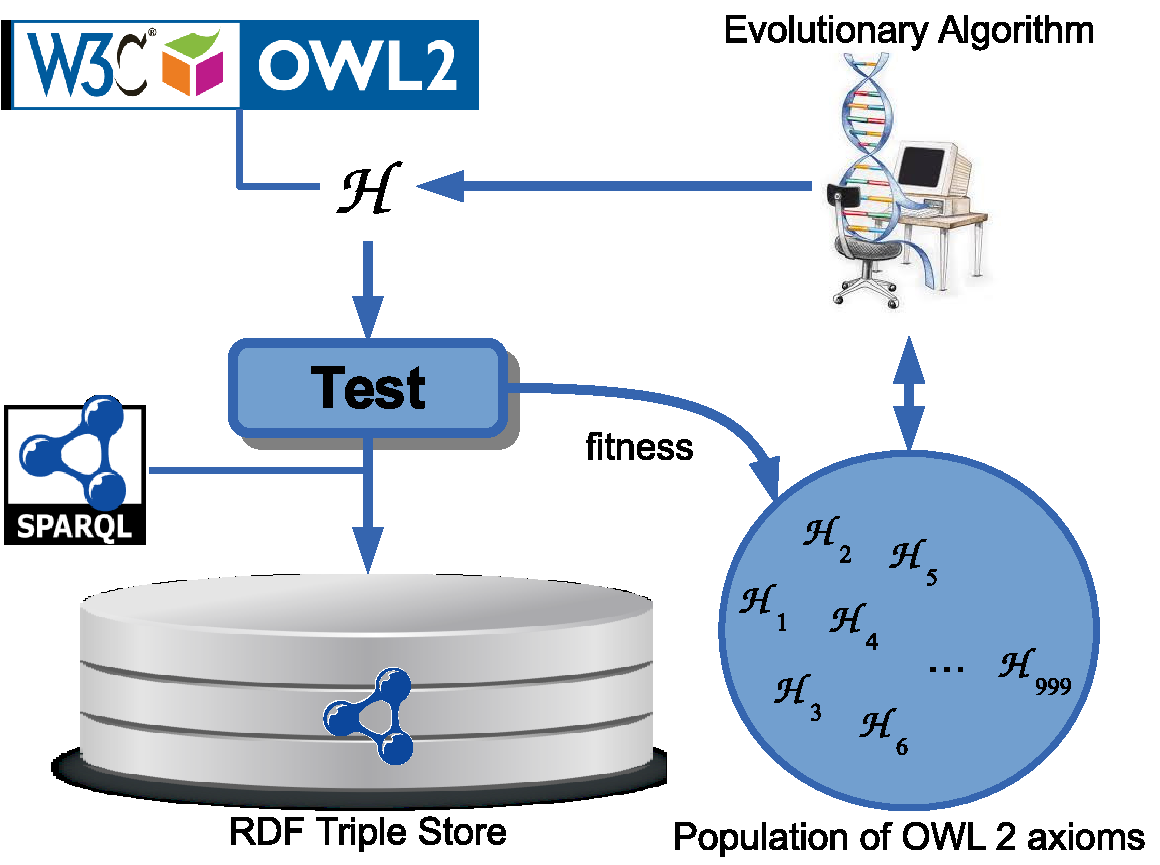
\includegraphics[height=2in]{synopsis}
  \end{center}
  \caption{A schematic illustration of the proposed approach.\label{fig:synopsis}}
\end{figure}



Possible applications of our research are:
\begin{itemize}
\item knowledge extraction from LOD in domains like genomics and proteomics;
\item providing tools to assist in the cleaning and validation of LOD;
\item information intelligence and the monitoring of strategic information on the LOD
  (this is linked with the problem of making sense of weak signals,
  weak signal interpretation).
\end{itemize}

\section{Survey of the Literature}
\label{sec:survey}

An early survey on Semantic Web Mining, dating from 2006, is the article by
Stumme, Hotho and Berendt~\cite{StummeHothoBerendt2006}.
Among the early approaches to what might be generally called ``ontology learning'',
which can go from the simple extraction of schema information all the way to the
induction of description logic TBoxes, we can mention
\begin{itemize}
\item the extraction of RDF schemas by systematic generalization~\cite{DelteilFaronDieng2001};
\item approaches based on clustering~\cite{MaedcheZacharias2002};
\item KAON Text-to-Onto, a framework that supports a semi-automatic, cooperative
  ontology engineering process~\cite{MaedcheStaab2004};
\item approaches based on inductive logic programming~\cite{GrimnesEdwardsPreece2004,FanizziDAmatoEsposito2008,Lehmann2009,dAmatoFanizziEsposito2010swj}.
\end{itemize}

A somehow related task is \emph{ontology alignment} or \emph{mapping},
whose aim is to establish equivalences among concepts defined in independent ontologies.
Extensional (i.e., instance-based) approaches to this task, such as
BLOOMS~\cite{JainHitzlerShethVermaYeh2010}
and BLOOMS+~\cite{JainYehVermaVasquezDamovaHitzlerSheth2011},
or AgreementMaker~\cite{CruzPalmonariCaimiStroe2013}
are of particular interest here.
Indeed, a recent approach to generate alignments between concepts
in ontologies of linked data sources, which looks at not only existing concepts,
but also at new hypothetical concepts defined using conjunctions and
disjunctions of (RDF) types and value restrictions~\cite{ParundekarKnoblockAmbite2012},
is just a little step away from outright ontology learning.
Slightly different approaches are
GLUE~\cite{DoanMadhavanDomingosHalevy2004}
and CSR~\cite{SpiliopoulosValarakosVouros2008},
which make use of machine-learning algorithms to predict the relationships
between concepts and their instances.

After the adoption by the W3C of OWL as an ontology language and of description logics
as its theoretical foundation, a number of approaches have been developed to automatically
identify concepts and produce their descriptions in such formalisms, like
\cite{HellmannLehmannAuer2009}, based on DL-Learner~\cite{Lehmann2009}.
See also the PhD Thesis of Claudia d'Amato on similarity-based learning
methods for the Semantic Web~\cite{dAmato2007} and her subsequent work with
Floriana Esposito and Steffen Staab and, in particular DL-FOIL~\cite{FanizziDAmatoEsposito2008}.

Another interesting research direction is to apply statistical schema induction
to enrich the schema of any RDF repository with property axioms. This is what is
done by Johanna V\"olker and colleagues~\cite{FleischhackerVoelkerStuckenschmidt2012},
who use association rule mining methods to induce property axioms in the RL fragment
of OWL (based on the $\mathcal{SROIQ}$ description logic) from RDF datasets.

A statistical approach to inferring RDF triples of the form $x \mathtt{rdf:type} y$
is also presented in \cite{PaulheimBizer2013}, based on the observed statistical
distribution of types in the subject and object positions of other properties.

The integration of traditional Semantic Web techniques and machine-learning-based
statistical inferencing motivates projects like
\href{https://files.ifi.uzh.ch/ddis/oldweb/ddis/research/completed-projects/semweb/sparql-ml/}{SPARQL-ML} \cite{KieferBernsteinLocher2008}.

\section{Targets for Inductive Learning in RDF Mining}

There are many possible targets (i.e., things to learn) for inductive learning from RDF data
which have been addressed in the literature.
These may be classified as concept-centric, property-centric, or instance-centric.

Concept-centric targets include
\begin{itemize}
\item concept induction/discovery;
\item concept subsumption;
\item concept disjointness.
\end{itemize}

Property-centric targets include
\begin{itemize}
\item property induction/discovery;
\item property subsumption;
\item domain restrictions;
\item range restrictions;
\item property disjointness;
\item algebraic properties of RDF properties, such as reflexivity, symmetry, transitivity,
  and functionality.
\end{itemize}

Instance-centric targets include
\begin{itemize}
\item predicting RDF triples in incomplete knowledge bases
(cf., e.g., \cite{DrumondRendleSchmiedtThieme2012}).
\end{itemize}

In addition to the above targets, a very hot current topic in the Semantic Web is
\emph{provenance}, i.e., taking the source of RDF data into account. In this
context, an interesting task would be to mine the RDF triples concerning provenance
to discover, e.g., cultural bias in DBpedia in different languages.

We will adopt as the target of our research the discovery of general OWL~2 axioms,
which may be seen as a generalization of all the learning targets listed above.
This is a very ambitious target and, to achieve it, we will have to combine a wide range
of results and techniques from various areas of machine learning, logic, and philosophy.
In particular, we will exploit ideas from inductive logic programming,
evolutionary computation, possibility theory, and epistemology.

\section{Background Notions from Inductive Logic Programming}
\label{ILP}

Inductive Logic Programming (ILP) is a research area which essentially combines
machine learning with logical knowledge representation to devise a formal framework
and practical algorithms for inductively learning logic programs
(e.g., in languages like Prolog or Datalog) from examples.
A good, if a little outdated, reference to ILP is the book by Lavra\v c and D\v zeroski~\cite{LavracDzeroski1994}; an account of the first twenty years of development of ILP
can be found in \cite{ILPat20}.

The problem of learning logic programs from examples can be viewed as a search problem
in the space of all possible hypotheses. Given a background knowledge, a set of positive
examples and a set of negative examples, expressed in some logical language,
one has to find a hypothesis which covers all positive examples and none of the negative ones.
This problem is NP-hard even if the language to represent hypotheses is propositional logic.
When hypotheses in an expressive language are used, this complexity is combined
with the complexity of evaluating hypotheses.

Although at the beginning the emphasis of ILP was on the inductive synthesis of logic programs,
what defines and unifies most of contemporary ILP is the relational form of the input,
rather than the logical language used to express the output \cite{ILPat20}.
Since ILP underlies most of the research efforts towards the extraction of knowledge from
RDF data, we will recall here some fundamental definitions and results which will be used
as a foundation for building our approach.

\subsection{Coverage}

Intuitively, coverage in ILP is the relationship between a hypothesis and an example,
whereby the example provides evidence in favor of the hypothesis. In that case,
one says that the hypothesis \emph{covers} the example.

Three views on coverage may be distinguished in ILP that are applicable to different
types of data, and ultimately stem from the distinction between the model-theoretic and
proof-theoretic perspectives in logic:
\begin{enumerate}
\item \emph{learning from interpretations} ---
  an example is a logical interpretation $\mathcal{I}$ and an example is covered
  by a hypothesis, which is a logical formula $\phi$, if $\mathcal{I} \models \phi$,
  i.e., $\mathcal{I}$ is a model for $\phi$;
\item \emph{learning from entailment} ---
  an example corresponds to an observation about the truth value of a formula $F$ (a fact)
  and a hypothesis $\phi$ covers the formula $F$ if $\phi \models F$,
  i.e. $\phi$ entails $F$;
\item \emph{learning from proofs} ---
  an example is a proof (or a trace of execution of a logic program)
  and an example $P$ is covered by hypothesis $\phi$ if $P$ is
  a possible proof in the hypothesis $\phi$.
\end{enumerate}
For our purposes, the \emph{learning from entailment} view is the most appropriate:
we have a set of facts, in the form of RDF triples or sets of RDF triples,
and our hypotheses will be formulas in a decidable fragment of first-order logic
(i.e., in a description logic language).

In fact, we will adopt yet another view, which does not fit exactly the orthodox ILP
framework, and stems from our adoption of possibility theory to take data imperfection
into account. We will regard the entire RDF repository as a set of interpretations
(the set of all interpretations $\mathcal{I}$ that agree with all the facts contained in it)
and we will say that a hypothesis is \emph{possible} if there exists a model for it within
that set and \emph{necessary} if all interpretations that agree with the known facts
are models for it. See Section~\ref{possibility-theory} for further details.

TO DO: DEFINE INTENSIONAL AND EXTENSIONAL COVERAGE

\subsection{Structure of the Hypothesis Space}

When hypotheses are logical formulas, the generality relation coincides with that
of logical entailment. A hypothesis $\phi$ is said to be more general than a hypothesis $\psi$
if $\phi \models \psi$. Applying a deductive inference operator leads to specializations,
whereas applying an inverted deductive operator leads to generalizations.
Many generalization and specialization operators have been proposed and theoretically studied
in the framework of ILP and their properties are well understood.

TO DO: THE STRUCTURE OF THE HYPOTHESIS SPACE

\subsection{Fundamental Techniques}

The hypothesis space can be searched from the bottom up or from the top down.
Generalization techniques proceed from the most specific hypothesis that covers a
given known fact and generalize it until it cannot be further generalized without
covering a counterexample.
Specialization techniques proceed from the most general hypotheses and refine them
until they no longer cover counterexamples.

INTRODUCE THE BASIC ILP GENERALIZATION AND SPECIALIZATION TECHNIQUES

Generalization and refinement operators will be used in our approach to add intelligent
mutation operators to the evolutionary algorithm in charge of exploring the hypothesis
space (see Section~\ref{EA})

The approach we will propose in the following sections may be classified as a
batch learner that learns multiple predicates; however, it incorporates some aspects
of interactive ILP, because it can be used to build a system that accepts an initial theory,
in the form of an existing ontology, and revises and corrects it based on the contents
of an RDF repository; furthermore, it may use the deductive power of an inference engine
coupled with an existing ontology as an oracle to answer membership queries.

\section{OWL~2 Axiom Discovery}
\label{axiom-discovery}

To get started, we may target DBpedia, which is a rather rich collection of
facts extracted from the Wikipedia and represented as RDF triples.
DBpedia provides a public SPARQL endpoint  at \url{http://dbpedia.org/sparql}
that can be used to query it.

Why DBPedia?
Becuase it poses a number of interesting challenges:
\begin{enumerate}
\item it is one of the largest collections of RDF triples, which covers all possible
  topics; its encyclopedic character makes it a fascinating object of study for a
  knowldege extraction method;
\item due to its collaborative character, it is incomplete and ridden with inconsistencies
  and errors;
\item it is evolutionary: the facts change in time.
\end{enumerate}
Of course, nothing forbid to apply the approach we are developing to more restricted
domains. Examples of such RDF repositories which might be targeted include:
\begin{itemize}
\item the dataset published in RDF by INSEE, the French national bureau of statistics,
  which was one of the targets of the Datalift project, on an analogous dataset
  published by ISTAT, the Italian national bureau of statistics;
\item a genomic or proteomic RDF datasets from Bioportal;
\item RDF data on TV broadcast programs, like those published by the BBC;
\end{itemize}
and possibly others.

Why OWL~2 axioms?
Because we are interested not only in extracting new knowledge from an existing knowledge
base expressed in RDF, but also in being able to inject such extracted knowledge into
an ontology in order to be able to use it to infer its logical consequences.
While the former objective calls for a target language, used to express the extracted
knowledge, which is as expressive as possible, lest we throttle our method,
the latter objective requires using at most a decidable fragment of first-order logic
and, possibly, a language which makes inference problems tractable.
OWL~2 represents a good compromise between these two objectives and one which, in addition,
is standardized and promotes interoperability with different applications.
Furthermore, depending on the applications, it will be possible to select an appropriate
\emph{profile} (corresponding to a different language fragment) exhibiting the
desired trade-off between expressiveness and computational complexity.

\subsection{Generating Hypotheses}
\label{generating-hypotheses}

The first step is to generate hypotheses, in the form of OWL~2 axioms.
The generated axioms may be general OWL~2 axioms or be restricted to a particular
fragment (called a \emph{profile}), depending on their intended use once they
are discovered.

The syntax of the logical language from which the axioms are to be
generated is given by a functional-style grammar expressed in the
\href{"http://www.w3.org/TR/2012/REC-owl2-syntax-20121211/#BNF_Notation}{extended BNF notation}
used by the \href{http://www.w3.org/}{W3C}.

The W3C tecnical recommendation \href{http://www.w3.org/TR/owl2-profiles}{OWL~2
Web Ontology Language Profiles} contains the productions of the functional-style syntax
that specify three \emph{profiles} (i.e., fragments) of the OWL~2 language,
namely, in increasing order of expressiveness, OWL 2 EL, OWL 2 QL, and OWL 2 RL.
% Catherine: I'm not sure this is really correct: one is not an extension of another.
The productions and, in general, the grammar specifications of OWL~2 and of its
fragments are published by the W3C in a quite easy-to-read notation which, however,
does not correspond neither to pure BNF,
nor to \href{http://tools.ietf.org/html/rfc5234}{ABNF},
nor to \href{http://www.w3.org/TR/xquery/#EBNFNotation}{EBNF},
the standard W3C grammar notation,
nor to any standardized grammar notation that we are aware of.
The conventions used are the following:
\begin{center}
  \begin{tabular}{|l|l|l|}
  \hline
    \sc Construct & \sc Syntax & \sc Example \\
  \hline
    production           & \texttt{:=}     & \textbf{Class} \texttt{:=} \textbf{IRI} \\
    non-terminal symbols & boldface        & \textbf{ClassExpression} \\
    terminal symbols     & single quoted   & \texttt{'PropertyRange'} \\
    zero or more         & curly braces    & \{ \textbf{ClassExpression} \} \\
    zero or one          & square brackets & [ \textbf{ClassExpression} ] \\
    alternative          & vertical bar    & \textbf{Assertion} $\mid$ \textbf{Declaration} \\
    grouping             & parentheses     & \textbf{dataPropertyExpression} ) \\
  \hline
  \end{tabular}
\end{center}

Not all of the productions contained in the official W3C grammar of OWL~2 need be
considered in order to generate axioms. The reason is here we are not using a grammar
to \emph{define} what a well-formed axiom may be; we are using it to \emph{generate}
axioms that may describe the facts contained in a given RDF tripe store. Therefore,
only resources, literals, properties, and other elements of the language that actually
occur in the RDF repository should be generated.

We solve this issue as follows:
\begin{itemize}
\item a \emph{static} grammar, containing high-level production rules defining the
  structure of the axioms is loaded from a text file; different grammars may be
  prepared to generate different kinds of axioms; such grammars need not define
  low-level non-terminal symbols, which we will call \emph{primitives};
\item production rules for the primitives are constructed at runtime by querying
  the SPARQL endpoint of the RDF repository; they constitute the \emph{dynamic}
  part of the grammar and ensure that the approach is not left behind as the
  contents of the RDF repository evolve or that different RDF repositories can
  be targeted without having to rewrite the grammar.
\end{itemize}
The primitives are the following:
\begin{itemize}
\item \texttt{Class} --- the IRI of a class mentioned in the RDF store,
  including \texttt{owl:Thing};
\item \texttt{Class-other-than-owl:Thing} --- the IRI of a class mentioned
  in the RDF store, except \texttt{owl:Thing} (this primitive is needed to define
  some OWL~2 profiles, although it is not part of OWL~2 full);
\item \texttt{ObjectProperty} --- the IRI of an object property used in the
  RDF store;
\item \texttt{DataProperty} --- the IRI of a data property used in the RDF store;
\item \texttt{NamedIndividual} --- the IRI of an individual occurring in the RDF store
  (anonymous individuals are defined by productions in the static grammar);
\item \texttt{Literal} --- any literal occurring in the RDF store
  % Catherine:
  (we do not have to check the construction of a literal like in the OWL~2 grammar);
\end{itemize}

\subsubsection{Static Productions}

The following is an EBNF grammar (in the format used in W3C documentation)
for constructing the fullest gamut of OWL~2 axioms.
The production rules are extracted and adapted from the complete normative grammar
of OWL~2 which can be found in the appendix of W3C technical recommendation
\href{http://www.w3.org/TR/2012/REC-owl2-syntax-20121211/}{OWL~2 Web Ontology Language
Structural Specification and Functional-Style Syntax (Second Edition)}.
\begin{enumerate}
\item Target production:
{\small
\begin{verbatim}
Axiom := ClassAxiom | ObjectPropertyAxiom | DataPropertyAxiom | HasKey | Assertion
\end{verbatim}
}
\item Axiom-level productions:
{\scriptsize
\begin{verbatim}
ClassAxiom := SubClassOf | EquivalentClasses | DisjointClasses | DisjointUnion
SubClassOf := 'SubClassOf' '(' subClassExpression ' ' superClassExpression ')'
subClassExpression := ClassExpression
superClassExpression := ClassExpression
EquivalentClasses := 'EquivalentClasses' '(' ClassExpression ' ' ClassExpression { ' ' ClassExpression } ')'
DisjointClasses := 'DisjointClasses' '(' ClassExpression ' ' ClassExpression { ' ' ClassExpression } ')'
DisjointUnion := 'DisjointUnion' '(' Class ' ' disjointClassExpressions ')'
disjointClassExpressions := ClassExpression ' ' ClassExpression { ' ' ClassExpression }

ObjectPropertyAxiom := SubObjectPropertyOf | EquivalentObjectProperties | DisjointObjectProperties |
  InverseObjectProperties | ObjectPropertyDomain | ObjectPropertyRange | FunctionalObjectProperty |
  InverseFunctionalObjectProperty | ReflexiveObjectProperty | IrreflexiveObjectProperty |
  SymmetricObjectProperty | AsymmetricObjectProperty | TransitiveObjectProperty
SubObjectPropertyOf := 'SubObjectPropertyOf' '(' subObjectPropertyExpression ' ' superObjectPropertyExpression ')'
subObjectPropertyExpression := ObjectPropertyExpression | propertyExpressionChain
propertyExpressionChain := 'ObjectPropertyChain' '(' ObjectPropertyExpression ' '
  ObjectPropertyExpression { ' ' ObjectPropertyExpression } ')'
superObjectPropertyExpression := ObjectPropertyExpression
EquivalentObjectProperties := 'EquivalentObjectProperties' '(' ObjectPropertyExpression ' '
  ObjectPropertyExpression { ' ' ObjectPropertyExpression } ')'
DisjointObjectProperties := 'DisjointObjectProperties' '(' ObjectPropertyExpression ' '
  ObjectPropertyExpression { ' ' ObjectPropertyExpression } ')'
ObjectPropertyDomain := 'ObjectPropertyDomain' '(' ObjectPropertyExpression ' ' ClassExpression ')'
ObjectPropertyRange := 'ObjectPropertyRange' '(' ObjectPropertyExpression ' ' ClassExpression ')'
InverseObjectProperties := 'InverseObjectProperties' '(' ObjectPropertyExpression ' ' ObjectPropertyExpression ')'
FunctionalObjectProperty := 'FunctionalObjectProperty' '(' ObjectPropertyExpression ')'
InverseFunctionalObjectProperty := 'InverseFunctionalObjectProperty' '(' ObjectPropertyExpression ')'
ReflexiveObjectProperty := 'ReflexiveObjectProperty' '(' ObjectPropertyExpression ')'
IrreflexiveObjectProperty := 'IrreflexiveObjectProperty' '(' ObjectPropertyExpression ')'
SymmetricObjectProperty := 'SymmetricObjectProperty' '(' ObjectPropertyExpression ')'
AsymmetricObjectProperty := 'AsymmetricObjectProperty' '(' ObjectPropertyExpression ')'
TransitiveObjectProperty := 'TransitiveObjectProperty' '(' ObjectPropertyExpression ')'

DataPropertyAxiom := SubDataPropertyOf | EquivalentDataProperties | DisjointDataProperties |
  DataPropertyDomain | DataPropertyRange | FunctionalDataProperty
SubDataPropertyOf := 'SubDataPropertyOf' '(' subDataPropertyExpression ' ' superDataPropertyExpression ')'
subDataPropertyExpression := DataPropertyExpression
superDataPropertyExpression := DataPropertyExpression
EquivalentDataProperties := 'EquivalentDataProperties' '(' DataPropertyExpression ' '
  DataPropertyExpression { ' ' DataPropertyExpression } ')'
DisjointDataProperties := 'DisjointDataProperties' '(' DataPropertyExpression ' '
  DataPropertyExpression { ' ' DataPropertyExpression } ')'
DataPropertyDomain := 'DataPropertyDomain' '(' DataPropertyExpression ' ' ClassExpression ')'
DataPropertyRange := 'DataPropertyRange' '(' DataPropertyExpression ' ' DataRange ')'
FunctionalDataProperty := 'FunctionalDataProperty' '(' DataPropertyExpression ')'

HasKey := 'HasKey' '(' ClassExpression '(' { ObjectPropertyExpression } ')' '(' { DataPropertyExpression } ')' ')'

Assertion := SameIndividual | DifferentIndividuals | ClassAssertion | ObjectPropertyAssertion |
 NegativeObjectPropertyAssertion | DataPropertyAssertion | NegativeDataPropertyAssertion
SameIndividual := 'SameIndividual' '(' Individual ' ' Individual { ' ' Individual } ')'
DifferentIndividuals := 'DifferentIndividuals' '(' Individual ' ' Individual { ' ' Individual } ')'
ClassAssertion := 'ClassAssertion' '(' ClassExpression ' ' Individual ')'
ObjectPropertyAssertion := 'ObjectPropertyAssertion' '(' ObjectPropertyExpression ' '
  Individual ' ' Individual ')'
NegativeObjectPropertyAssertion := 'NegativeObjectPropertyAssertion' '(' ObjectPropertyExpression ' '
  Individual ' ' Individual ')'
DataPropertyAssertion := 'DataPropertyAssertion' '(' DataPropertyExpression ' '
  Individual ' ' Literal ')'
NegativeDataPropertyAssertion := 'NegativeDataPropertyAssertion' '(' DataPropertyExpression ' '
  Individual ' ' Literal ')'
\end{verbatim}
}
\item Expression-level productions:
{\scriptsize
\begin{verbatim}
ObjectPropertyExpression := ObjectProperty | InverseObjectProperty
InverseObjectProperty := 'ObjectInverseOf' '(' ObjectProperty ')'

DataPropertyExpression := DataProperty

DataRange :=  Datatype | DataIntersectionOf | DataUnionOf | DataComplementOf |  DataOneOf | DatatypeRestriction
Datatype := 'rdfs:Literal' | 'owl:rational' | 'owl:real' | 'xsd:double' | 'xsd:float' | 'xsd:decimal' |
  'xsd:integer' | 'xsd:long' | 'xsd:int' | 'xsd:short' | 'xsd:byte' | 'xsd:nonNegativeInteger' |
  'xsd:nonPositiveInteger' | 'xsd:positiveInteger' | 'xsd:negativeInteger' | 'xsd:unsignedLong' |
  'xsd:unsignedInt' | 'xsd:unsignedShort' | 'xsd:unsignedByte' | 'rdf:PlainLiteral' | 'xsd:string' |
  'xsd:NCName' | 'xsd:Name' | 'xsd:NMTOKEN' | 'xsd:token' | 'xsd:language' | 'xsd:normalizedString' |
  'xsd:boolean' | 'xsd:base64Binary' | 'xsd:hexBinary' | 'xsd:anyURI' | 'xsd:dateTime' | 'xsd:dateTimeStamp' |
  'rdf:XMLLiteral'
DataIntersectionOf := 'DataIntersectionOf' '(' DataRange ' ' DataRange { ' ' DataRange } ')'
DataUnionOf := 'DataUnionOf' '(' DataRange ' ' DataRange { ' ' DataRange } ')'
DataComplementOf := 'DataComplementOf' '(' DataRange ')'
DataOneOf := 'DataOneOf' '(' Literal { ' ' Literal } ')'
DatatypeRestriction := 'DatatypeRestriction' '(' Datatype ' ' Facet ' ' Literal { ' ' Facet ' ' Literal } ')'
Facet := 'xsd:minInclusive' | 'xsd:maxInclusive' | 'xsd:minExclusive' | 'xsd:maxExclusive' |
  'xsd:minLength' | 'xsd:maxLength' | 'xsd:length' | 'xsd:pattern' | 'rdf:langRange'

ClassExpression := Class |
  ObjectIntersectionOf | ObjectUnionOf | ObjectComplementOf | ObjectOneOf |
  ObjectSomeValuesFrom | ObjectAllValuesFrom | ObjectHasValue | ObjectHasSelf |
  ObjectMinCardinality | ObjectMaxCardinality | ObjectExactCardinality |
  DataSomeValuesFrom | DataAllValuesFrom | DataHasValue |
  DataMinCardinality | DataMaxCardinality | DataExactCardinality
ObjectIntersectionOf := 'ObjectIntersectionOf' '(' ClassExpression ' ' ClassExpression
  { ' ' ClassExpression } ')'
ObjectUnionOf := 'ObjectUnionOf' '(' ClassExpression ' ' ClassExpression { ' ' ClassExpression } ')'
ObjectComplementOf := 'ObjectComplementOf' '(' ClassExpression ')'
ObjectOneOf := 'ObjectOneOf' '(' Individual { ' ' Individual }')'
ObjectSomeValuesFrom := 'ObjectSomeValuesFrom' '(' ObjectPropertyExpression ' ' ClassExpression ')'
ObjectAllValuesFrom := 'ObjectAllValuesFrom' '(' ObjectPropertyExpression ' ' ClassExpression ')'
ObjectHasValue := 'ObjectHasValue' '(' ObjectPropertyExpression ' ' Individual ')'
ObjectHasSelf := 'ObjectHasSelf' '(' ObjectPropertyExpression ')'
ObjectMinCardinality := 'ObjectMinCardinality' '(' nonNegativeInteger ' ' ObjectPropertyExpression
  [ ' ' ClassExpression ] ')'
ObjectMaxCardinality := 'ObjectMaxCardinality' '(' nonNegativeInteger ' ' ObjectPropertyExpression
  [ ' ' ClassExpression ] ')'
ObjectExactCardinality := 'ObjectExactCardinality' '(' nonNegativeInteger ' ' ObjectPropertyExpression
  [ ' ' ClassExpression ] ')'
DataSomeValuesFrom := 'DataSomeValuesFrom' '(' DataPropertyExpression { ' ' DataPropertyExpression }
  ' ' DataRange ')'
DataAllValuesFrom := 'DataAllValuesFrom' '(' DataPropertyExpression { ' ' DataPropertyExpression }
  ' ' DataRange ')'
DataHasValue := 'DataHasValue' '(' DataPropertyExpression ' ' Literal ')'
DataMinCardinality := 'DataMinCardinality' '(' nonNegativeInteger ' ' DataPropertyExpression
  [ ' ' DataRange ] ')'
DataMaxCardinality := 'DataMaxCardinality' '(' nonNegativeInteger ' ' DataPropertyExpression
  [ ' ' DataRange ] ')'
DataExactCardinality := 'DataExactCardinality' '(' nonNegativeInteger ' ' DataPropertyExpression
  [ ' ' DataRange ] ')'

nonNegativeInteger := '0' | '1' | '2' | '3' | '4' | '5' | '6' | '7' | '8' | '9' | '10' | '11' | '12'

Individual := NamedIndividual | AnonymousIndividual
AnonymousIndividual := '_:' LowerCaseLetter
LowerCaseLetter := 'a' | 'b' | 'c' | 'd' | 'e' | 'f' | 'g' | 'h' | 'i' | 'j' | 'k' | 'l' |
  'm' | 'n' | 'o' | 'p' | 'q' | 'r' | 's' | 't' | 'u' | 'v' | 'w' | 'x' | 'y' | 'z'
\end{verbatim}
}
\end{enumerate}
Since it would not make sense to generate axiom annotations, all symbols and productions
related to annotations have been removed. Ditto for datatype definitions: we are going
to refer to built-in datatypes only, or, at most, to datatypes that are actually used
in the RDF repository; it would not be interesting to define new datatypes. The same
applies also to facets.
All symbols and productions related to declarations have been removed as well, for the same reason.

Notice also that the definitions of the \texttt{nonNegativeInteger} and \texttt{AnonymousIndividual}
non-terminal symbols are simplifications suited to the needs of this project, as are
the productions for \texttt{Datatype} and \texttt{Facet}, which only take into account
built-in datatypes and facets, respectively.

\subsubsection{Dynamic Productions}

The SPARQL queries used to construct the productions for the six primitives are
the following.
\begin{itemize}

\item For the \texttt{Class} primitive:
\begin{verbatim}
SELECT DISTINCT ?class WHERE { ?_ a ?class }\end{verbatim}

\item For the \texttt{Class-other-than-owl:Thing} primitive, not used in the general
grammar of OWL~2 full, but needed to define some of the OWL~2 profiles, we use the same
query, by adding a filter constraint:
\begin{verbatim}
SELECT DISTINCT ?class WHERE {
  ?_ a ?class .
  FILTER ( ?class != owl:Thing )
}\end{verbatim}

\item For the \texttt{ObjectProperty} primitive, we select the properties whose
fillers are individuals (WHAT ABOUT BLANK NODES AS FILLERS?),
i.e., RDF resources, represented by IRIs:
\begin{verbatim}
SELECT DISTINCT ?prop WHERE {
  ?subj ?prop ?obj .
  FILTER ( isIRI(?obj) )
}\end{verbatim}
To include properties whose fillers are blank nodes, the filter would have to be
changed into \texttt{isIRI(?obj) || isBlank(?obj)}.

\item For the \texttt{DataProperty} primitive, we select the properties whose values
are literals:
\begin{verbatim}
SELECT DISTINCT ?prop WHERE {
  ?subj ?prop ?obj
  FILTER ( isLiteral(?obj) )
}\end{verbatim}

\item For the \texttt{NamedIndividual} primitive, we gather all RDF resources $x$ which
appear as the subject of a triple of the form $x$ \texttt{rdf:type} \textit{class}:
\begin{verbatim}
SELECT DISTINCT ?ind WHERE { ?ind a ?class . FILTER ( isIRI(?ind) ) }\end{verbatim}
Admittedly, this might be regarded as a rather restrictive criterion, for other individuals
might appear in the RDF store only as the subject or the object of a triple, i.e., as role fillers, without
their membership in a class being declared. If we wanted to include these individuals too,
we would have to replace the above query with something like
\begin{verbatim}
SELECT DISTINCT ?ind WHERE {
  { ?ind a ?class .
    FILTER ( isIRI(?ind) )
  }
  UNION {
    ?ind ?prop ?obj
    FILTER ( isIRI(?ind) )
  }
  UNION {
    ?subj ?prop ?ind .
    FILTER ( isIRI(?ind) )
  }
}\end{verbatim}

\item For the \texttt{Literal} primitive, we may use exactly the same graph pattern as for
the \texttt{DataProperty} query, except that we now project on the \texttt{?obj} variable,
since literals only appear as objects of RDF triples:
\begin{verbatim}
SELECT DISTINCT ?obj WHERE {
  ?subj ?prop ?obj
  FILTER ( isLiteral(?obj) )
}\end{verbatim}

\end{itemize}
The lists of solutions $s_1, s_2, \ldots, s_n$ returned by the above queries
for each primitive $P$ are used to add new productions to the grammar of the form
\begin{quote}
  $P$ \texttt{:=} $s_1$ \texttt{|} $s_2$ \texttt{|} $\ldots$ \texttt{|} $s_n$.
\end{quote}
This tends to produce very large grammars which are sort of \emph{flat}, i.e., consisting of
a huge number of simple productions alongside with a small number of more complex productions.
These grammars use up some memory space, but lead to relatively shallow derivation trees
and are therefore quite efficient for the purpose of generating axioms.

\subsection{Induction from an Epistemological Perspective}
\label{epistemology}

Discovering axioms from a finite, albeit huge, set of known facts
raises philosophical problems that touch upon the discipline of epistemology.
The task may be regarded as a form of inductive reasoning, in that it proceeds
from particular instances of concepts and relations (the RDF triples)
to broader generalizations (the OWL~2 axioms).
At the same time, machine learning provides the theoretical and practical
framework within which the task of axiom induction from RDF triples
should be addressed algorithmically.

The \emph{problem of induction} is the question whether, or under which conditions,
and to what degree, inductive inferences are justified.
A very influential, if controversial, view on such problem, and one which seems
particularly well-suited to the context of axiom induction from RDF repositories,
is Karl Popper's evolutionary approach to epistemology. As a matter of fact,
we might say that Popper's point of view is that the problem of induction is ill-posed.
His solution to the problem is to reject induction as useless and to propose the principle
of \emph{falsifiability} \cite{Popper1935}, which lies at the foundation of his critical rationalism:
all knowledge is provisional, conjectural, hypothetical---we can never finally
prove our scientific theories, we can merely (provisionally) confirm or
(conclusively) refute them.

In Popper's view, the advance of scientific knowledge is an evolutionary process~\cite{Popper1972}
whereby, prompted by a problem, a number of competing conjectures, or tentative theories,
are proposed and systematically subjected to a process of error elimination,
a rigorous scrutiny, whose aim is to falsify them, i.e., to find facts (observations,
results experiments) that show them to be false.
This process performs a similar function for Science that natural selection performs
for biological evolution. Theories that better survive the process of refutation
are not more true, but rather, more ``fit'', i.e., more suited to solving
the problem at hand.
However,
\begin{quote}
while falsifiability is simple as a logical principle, in practice it is exceedingly
complicated---no single observation can ever be taken to falsify a theory,
for there is always the possibility (a) that the observation itself is mistaken,
or (b) that the assumed background knowledge is faulty or defective \cite{Thornton2013}.
\end{quote}

It should be said that Popper made his proposal within the context of Philosophy of Science
and, within this context, his ideas have later been refined and extended by other
philosphers, like Imre Lakatos~\cite{Lakatos1976}, and challenged and superseded by others,
like Thomas Kuhn~\cite{Kuhn1962} and Paul Feyerabend~\cite{Feyerabend1975}.
However, if we abstract them from the specific context of scientific discovery
and we regard them as a tentative explanation of how knowledge may be expanded
through the observation of facts, their value as a source of inspiration cannot be denied.

This philosophical synthesis of Darwinism and epistemology, initiated by Popper,
has been called \emph{evolutionary epistemology} by Donald Campbell~\cite{Campbell1974}.
Evolutionary Epistemology is a naturalistic approach to epistemology,
which appeals to natural selection in two roles~\cite{BradieHarms2012}:
\begin{enumerate}
\item selection is the reason for the general reliability of our ``common sense''
  and our cognitive mechanisms;
\item trial and error learning and the evolution of scientific theories
  are construed as selection processes.
\end{enumerate}
Bradie~\cite{Bradie1986} has called Evolution of Epistemological Mechanisms (EEM)
the former and Evolutionary Epistemology of Theories the latter.

Popper introduces the concept of \emph{degree of verisimilitude}, which makes us think
of an attempt at something like possibility theory.
Too bad Popper was not aware of possibility theory, otherwise perhaps he could have used
this tool to describe his ideas.
A confirmation that what Popper calls ``degree of corroboration'' of a hypothesis
is to be regarded as a possibility measure is what Popper writes on Page~19,
item~4, of \cite{Popper1972}, which may be paraphrased as follows:
given a theory $T$ and a sentence $s$ (one of its consequences),
if $T \models s$, $\mathrm{corroboration}(s) \leq \mathrm{corroboration}(T)$
and
\[
  \mathrm{corroboration}(T) = \max_{T \models s} \mathrm{corroboration}(s).
\]

We can equate the axioms generated by our algorithm to conjectures, hypotheses
in Popper's terms, and facts contained in the RDF repository to observations,
``basic statements'' in Popper's terms.

We may define the statement that an observation refutes, or contradicts, a hypothesis
as equivalent to saying that a TBox containing the axiom corresponding to the hypothesis
and an ABox containing the assertion corresponding to the observation make an
inconsistent knowledge base.

While the definition of ``contradicts'' is clear enough not to be subject to debate,
defining what it means to ``confirm'' a hypothesis is much more tricky. This is
of course closely related to Popper's observation that a hypothesis can never be
conclusively confirmed.

The difficulty of finding a satisfactory and intuitive definition of confirmation
is witnessed by Hempel's ``black raven''paradox of confirmation~\cite{Hempel1945}:
if we suppose (i) that a simple universal condition (``all ravens are black'')
is satisfied by joint satisfaction of its antecedent and consequent, and we
also accept (ii) that whatever confirms a statement confirms also all its logical
equivalents (e.g., ``all non-black things are not ravens'') --- the \emph{equivalence hypothesis},
then we must conclude that a blue chair, for example, confirms the hypothesis
that all ravens are black.

The hypothesis ``all ravens are black'' may be
written $\mathsf{Raven} \sqsubseteq \mathsf{Black}$ in a description logic language.
This statement is logically equivalent to $\neg\mathsf{Black} \sqsubseteq \neg\mathsf{Raven}$.
The paradox arises from the fact that an observation of, say, a green apple,
may be taken as a confirmation of the latter statement and, therefore, by the
equivalence of the two statements, also of the hypothesis that all ravens are black,
even though it has nothing to do with ravens!

Although Hempel's solution of the paradox was to accept the paradoxical conclusion
and argue that our intuition is biased by our background knowledge, the most popular
solution is to approach it from a statistical point of view. The key of this solution
is to assign a weight to evidence in terms of the Bayes factor. Deciding whether
$\mathsf{Raven} \sqsubseteq \mathsf{Black}$ is true, rather than its contrary, on the basis
of some observed data $D$ may be stated as a model selection problem in which the two
``models'' may be assessed by the Bayes factor
\begin{equation}
  K = \frac{\Pr(D \mid \mathsf{Raven} \sqsubseteq \mathsf{Black})}{\Pr(D \mid \mathsf{Raven} \not\sqsubseteq \mathsf{Black})}.
\end{equation}
Then, observing a green apple does indeed confirm our hypothesis, but its weight
is much lower than observing a black raven, just because there are so many more non-ravens in the
Universe than ravens and so many colors those object can be of. This argument, which
is known as the Bayesian solution to Hempel's paradox, seems convincing enough,
but it cannot be blindly accepted in all contexts.

In fact, the key argument for rejecting a probabilistic approach (like the Bayesian solutions
or the Carnapian approach) in the specific context of axiom induction from an RDF store
like DBPedia, which contains facts automatically extracted from Wikipedia,
which is the result of a collaborative effort, whose coverage is not planned and
subject to cultural and historical biases \footnote{For example, at the level
of pop music, the coverage of DBpedia is very much biased towards anglophone artists.
EXPAND AND PROVIDE OTHER EXAMPLES. On the other hand, it is likely that the coverage
of DBpedia in certain domains, such as geographical data, be much more uniform and
extensive.}.
% Catherine: what is specific? Isn't it the case of all any data/knowledge base?
% If we speak about the entire LOD this may be different but this is not the case I suppose
Therefore, there is no reason to assume that the facts contained in an RDF triple store
be \emph{representative} of all possible facts that could be recorded, unless
that RDF store is the result of a planned and well-designed effort aimed at building
a knowledge base providing uniform coverage of a given domain.
Indeed, to use the number of facts supporting a hypothesis
to estimate its probability one would have to make the very strong assumption
that the finite number of recorded facts are randomly extracted, according to a
uniform distribution, from the infinite number of all ``real'' facts, whatever
this means. Adopting a probabilistic approach whereas its assumptions are not
fulfilled might lead to fallacious results.

Applying Popper's idea of falsifiability to the induction problem,
Scheffler and Goodman introduced the concept of \emph{selective confirmation}
\cite{SchefflerGoodman1972}, whereby evidence may be characterized
not simply as satisfying a hypothesis, but, further, as favoring the hypothesis
rather than its contrary.
Thus, evidence of a black raven \emph{selectively confirms} the hypothesis
$\mathsf{Raven} \sqsubseteq \mathsf{Black}$ because it fails to confirm its
negation, $\top \sqsubseteq \mathsf{Raven} \sqcap \neg\mathsf{Black}$, namely
that there exist ravens that are not black. On the contrary, the observation of
a green apple does not contradict $\mathsf{Raven} \sqsubseteq \mathsf{Black}$,
but it does not disconfirm $\top \sqsubseteq \mathsf{Raven} \sqcap \neg\mathsf{Black}$
either; therefore, it does not selectively confirm $\mathsf{Raven} \sqsubseteq \mathsf{Black}$.
Selective confirmation is a nice example of a definition of ``provides evidence in favor of,''
which does not coincide with or imply ``increases the probability of''.
Therefore, we will adopt such a definition of confirmation.

\subsection{Testing Hypotheses}

Conceptually, one could imagine generating all possible OWL~2 axioms (or axioms of
one of the OWL fragments) one by one,
checking each of them against the facts contained in the RDF repository (the ABox).
Of course, we should first complete the TBox with all the axioms that can be
logically inferred from the ones declared in the TBox by taking into account OWL~2 semantics.
Checking an axiom involves constructing one or more corresponding SPARQL queries,
as explained below, executing them and counting the number of confirmations and counterexamples.

This idea of testing OWL axioms is somehow related with approaches aiming at evaluating
the quality of linked data by regarding OWL axioms as integrity constraints.
Clarck and Parsia's Pellet integrity constraint validator (ICV) translates OWL integrity constraint
ontologies into SPARQL queries automatically to validate RDF data~\cite{SirinTao2009}.
A similar approach also underlies the idea of test-driven evaluation of linked data
quality~\cite{KontokostasWestphalAuerHellmannLehmannCornelissen2014}.
To this end, OWL ontologies are interpreted under the closed-world assumption and
the weak unique name assumption. OWL is, therefore, used as an RDF schema language.

What we want to do is the exact opposite: instead of starting from the \emph{a priori}
assumption that a given ontology is correct and verify whether the facts contained
in an RDF base satisfy it, we treat ontologies (and their axioms) like hypotheses and develop
a methodology to verify whether the RDF facts corroborate or falsify them under the
open-world assumption and without making the unique name assumption.

TO DO: CONSIDER THIS POSSIBLE COMPLICATION:
Once a hypothesis is ``accepted'' (considered to be true, or, as Popper would say, the best
available approximation to truth),
it may modify the result of another query testing another hypothesis.
It can also enable to logically infer new axioms in the TBox.
However appealing the idea of automatically extending an ontology may appear,
one should be aware of the dangers: permanently accepting an incorrect axiom and adding
it to an existing ontology might have far-reaching consequences on the subsequent search
for other axioms. One should never forget that all knowledge discovered from RDF data
is conjectural in character and has to be subjected to revision each time that the data
in the RDF repository change or better (i.e., more general, more precise, more falsifiable)
axioms are discovered.
SEE ALSO BELOW THE REMARK ON A POSSIBILISTIC ONTOLOGY.

OWL~2 provides for 32 types of axioms, that can be grouped in six categories:
\begin{enumerate}
\item class expression axioms:
  \begin{itemize}
  \item \textsf{SubClassOf} axioms;
  \item \textsf{EquivalentClasses} axioms;
  \item \textsf{DisjointClasses} axioms;
  \item \textsf{DisjointUnion} axioms;
  \end{itemize}
\item object property expression axioms:
  \begin{itemize}
  \item \textsf{SubObjectPropertyOf} axioms;
  \item \textsf{EquivalentObjectProperties} axioms;
  \item \textsf{DisjointObjectProperties} axioms;
  \item \textsf{ObjectPropertyDomain} axioms;
  \item \textsf{ObjectPropertyRange} axioms;
  \item \textsf{InverseObjectProperties} axioms;
  \item \textsf{FunctionalObjectProperty} axioms;
  \item \textsf{InverseFunctionalObjectProperty} axioms;
  \item \textsf{ReflexiveObjectProperty} axioms;
  \item \textsf{IrreflexiveObjectProperty} axioms;
  \item \textsf{SymmetricObjectProperty} axioms;
  \item \textsf{AsymmetricObjectProperty} axioms;
  \item \textsf{TransitiveObjectProperty} axioms;
  \end{itemize}
\item data property expression axioms:
  \begin{itemize}
  \item \textsf{SubDataPropertyOf} axioms;
  \item \textsf{EquivalentDataProperties} axioms;
  \item \textsf{DisjointDataProperties} axioms;
  \item \textsf{DataPropertyDomain} axioms;
  \item \textsf{DataPropertyRange} axioms;
  \item \textsf{FunctionalDataProperty} axioms;
  \end{itemize}
\item datatype definition, identified by the \textsf{DatatypeDefinition} keyword;
\item keys axioms, identified by the \textsf{HasKey} keyword;
\item assertions:
  \begin{itemize}
  \item \textsf{SameIndividual} axioms;
  \item \textsf{DifferentIndividuals} axioms;
  \item \textsf{ClassAssertion} axioms;
  \item \textsf{ObjectPropertyAssertion} axioms;
  \item \textsf{NegativeObjectPropertyAssertion} axioms;
  \item \textsf{DataPropertyAssertion} axioms;
  \item \textsf{NegativeDataPropertyAssertion} axioms.
  \end{itemize}
\end{enumerate}
We may refer to the OWL~2 direct semantics~\cite{OWL2-direct-semantics}
\footnote{\url{http://www.w3.org/TR/2012/REC-owl2-direct-semantics-20121211/}}
for a model-theoretic semantics of all the types of axioms, compatible with
the description logic $\mathcal{SROIQ}$~\cite{HorrocksKutzSattler2006}.

Before summarizing that semantics, let us explain how it will be used to
check axioms. A model-theoretic semantics defines a valuation function
$\cdot^\mathcal{I}$ which maps well-formed formulas of the logical language into
elements and sets of elements of the interpretation domain $\Delta^\mathcal{I}$.
We will take the set of all the resources that occur in a given RDF store
(for instance, DBpedia) as the interpretation domain and checking an axiom
will amount to checking whether the interpretation $\mathcal{I}$ with the
valuation function defined by the semantics and the domain given by the
RDF store is a model of the axiom.

However, unlike interpretations, RDF stores, or ABoxes, are incomplete and
possibly noisy. The open-world hypothesis must be made; therefore, absence of
supporting evidence does not necessarily contradict an axiom, and an axiom might
hold even in the face of a few counterexamples (exceptions or possible mistakes).
We will tackle this issue in Section~\ref{possibility-theory}.

We adopt the following conventions to name metavariables:
\begin{itemize}
\item $a$, $a_i$ denote individual names;
\item $C$, $C_i$ denote concept expressions (called \emph{class expressions} in OWL~2);
\item $D$, $D_i$ denote datatype expressions;
\item $\mathtt{D}$ is the concrete data domain
\item $d$, $d_i$ denote data literals;
\item $\Delta^\mathcal{I}$ is the interpretation domain;
\item $F$, $F_i$ denote \emph{facets};
\item $R$, $R_i$ denote relations (called \emph{properties} in OWL~2:
  \emph{object properties} are relations $R \subseteq \Delta^\mathcal{I} \times \Delta^\mathcal{I}$;
  \emph{data properties} are relations $R' \subseteq \Delta^\mathcal{I} \times \mathtt{D}$);
\end{itemize}

\subsection{Translating OWL~2 Expressions into SPARQL Graph Patterns}

Table~\ref{tab:term-semantics}, which corresponds to the
\href{http://www.w3.org/TR/2012/REC-owl2-direct-semantics-20121211/}{OWL~2 Web Ontology Language Direct Semantics},
provides a reference of the model-theoretic semantics
of the constructs that may be used to write term expressions in OWL~2.

\begin{table}
\caption{The model-theoretic semantics of the various constructs that may be used
to construct term expressions in the Web ontology language OWL~2.
The first column gives the functional-style OWL syntax of the expression,
the second column its more compact $\mathcal{SHOIQ}$ description logic syntax,
and the last column shows its semantics.\label{tab:term-semantics}}
\begin{center}
\begin{tabular}{|l|l|l|}
\hline
  OWL~2 (functional-style) & DL Syntax & Interpretation \\
\hline &&\\[-0.95em]\hline
  $\mathsf{ObjectInverseOf}(R)$ & $R^-$ &
    $(R^-)^\mathcal{I} = \{\langle y, x \rangle \mid \langle x, y \rangle \in R^\mathcal{I} \}$ \\
\hline
  $\mathsf{DataIntersectionOf}(D_1\ \ldots\ D_n)$ & $D_1 \sqcap \ldots \sqcap D_n$  &
    $D_1^\mathcal{I} \cap \ldots \cap D_n^\mathcal{I}$ \\
  $\mathsf{DataUnionOf}(D_1\ \ldots\ D_n)$ & $D_1 \sqcup \ldots \sqcup D_n$  &
    $D_1^\mathcal{I} \cup \ldots \cup D_n^\mathcal{I}$ \\
  $\mathsf{DataComplementOf}(D)$ & $\neg D$ & $\mathtt{D}^{\mathrm{arity}(D)} \setminus D^\mathcal{I}$ \\
  $\mathsf{DataOneOf}(d_1\ \ldots\ d_n)$ & $\{d_1, \ldots, d_n\}$ &
    $\{d_1^\mathcal{I}, \ldots, d_n^\mathcal{I}\}$ \\
  $\mathsf{DatatypeRestriction}(D\ F_1\ d_1\ \ldots\ F_n\ d_n)$ &  &
    $D^\mathcal{I} \cap \langle F_1, d_1\rangle^\mathcal{I} \cap \ldots \cap \langle F_n, d_n\rangle^\mathcal{I}$  \\
\hline
  $\mathsf{ObjectIntersectionOf}(C_1\ \ldots\ C_n)$ & $C_1 \sqcap \ldots \sqcap C_n$ &
    $C_1^\mathcal{I} \cap \ldots \cap C_n^\mathcal{I}$ \\
  $\mathsf{ObjectUnionOf}(C_1\ \ldots\ C_n)$ & $C_1 \sqcup \ldots \sqcup C_n$ &
    $C_1^\mathcal{I} \cup \ldots \cup C_n^\mathcal{I}$ \\
  $\mathsf{ObjectComplementOf}(C)$ & $\neg C$ & $\Delta^\mathcal{I} \setminus C^\mathcal{I}$ \\
  $\mathsf{ObjectOneOf}(a_1\ \ldots\ a_n)$ & $\{a_1, \ldots, a_n\}$ & $\{a_1^\mathcal{I}, \ldots, a_n^\mathcal{I}\}$ \\
  $\mathsf{ObjectSomeValuesFrom}(R\ C)$ & $\exists R.C$  &
    $\{x \mid \exists y.\langle x, y\rangle \in R^\mathcal{I} \land y \in C^\mathcal{I}\}$ \\
  $\mathsf{ObjectAllValuesFrom}(R\ C)$ & $\forall R.C$ &
    $\{x \mid \forall y.\langle x, y\rangle \in R^\mathcal{I} \Rightarrow y \in C^\mathcal{I}\}$ \\
  $\mathsf{ObjectHasValue}(R\ a)$ & $\exists R.\{a\}$ &
    $\{x \mid \langle x, a^\mathcal{I}\rangle \in R^\mathcal{I}\}$ \\
  $\mathsf{ObjectHasSelf}(R)$ & $\exists R.\mathsf{Self}$ &
    $\{x \mid \langle x, x\rangle \in R^\mathcal{I}\}$ \\
  $\mathsf{ObjectMinCardinality}(n\ R)$ & $\geq nR.\top$ &
    $\{x \mid \|\{y \mid \langle x, y\rangle \in R^\mathcal{I}\}\| \geq n\}$ \\
  $\mathsf{ObjectMaxCardinality}(n\ R)$ & $\leq nR.\top$ &
    $\{x \mid \|\{y \mid \langle x, y\rangle \in R^\mathcal{I}\}\| \leq n\}$ \\
  $\mathsf{ObjectExactCardinality}(n\ R)$ & $=nR.\top$ &
    $\{x \mid \|\{y \mid \langle x, y\rangle \in R^\mathcal{I}\}\| = n\}$ \\
  $\mathsf{ObjectMinCardinality}(n\ R\ C)$ & $\geq nR.C$ &
    $\{x \mid \|\{y \mid \langle x, y\rangle \in R^\mathcal{I} \land y \in C^\mathcal{I}\}\| \geq n\}$ \\
  $\mathsf{ObjectMaxCardinality}(n\ R\ C)$ & $\leq nR.C$ &
    $\{x \mid \|\{y \mid \langle x, y\rangle \in R^\mathcal{I} \land y \in C^\mathcal{I}\}\| \leq n\}$ \\
  $\mathsf{ObjectExactCardinality}(n\ R\ C)$ & $=nR.C$ &
    $\{x \mid \|\{y \mid \langle x, y\rangle \in R^\mathcal{I} \land y \in C^\mathcal{I}\}\| = n\}$ \\
\hline
  $\mathsf{DataSomeValuesFrom}(R\ D)$ & $\exists R.D$  &
    $\{x \mid \exists y.\langle x, y\rangle \in R^\mathcal{I} \land y \in D^\mathcal{I}\}$ \\
  $\mathsf{DataAllValuesFrom}(R\ D)$ & $\forall R.D$ &
    $\{x \mid \forall y.\langle x, y\rangle \in R^\mathcal{I} \Rightarrow y \in D^\mathcal{I}\}$ \\
  $\mathsf{DataHasValue}(R\ d)$ & $\exists R.d$ &
    $\{x \mid \langle x, d^\mathcal{I}\rangle \in R^\mathcal{I}\}$ \\
  $\mathsf{DataMinCardinality}(n\ R)$ & $\geq nR.\top$ &
    $\{x \mid \|\{y \mid \langle x, y\rangle \in R^\mathcal{I}\}\| \geq n\}$ \\
  $\mathsf{DataMaxCardinality}(n\ R)$ & $\leq nR.\top$ &
    $\{x \mid \|\{y \mid \langle x, y\rangle \in R^\mathcal{I}\}\| \leq n\}$ \\
  $\mathsf{DataExactCardinality}(n\ R)$ & $=nR.\top$ &
    $\{x \mid \|\{y \mid \langle x, y\rangle \in R^\mathcal{I}\}\| = n\}$ \\
  $\mathsf{DataMinCardinality}(n\ R\ D)$ & $\geq nR.D$ &
    $\{x \mid \|\{y \mid \langle x, y\rangle \in R^\mathcal{I} \land y \in D^\mathcal{I}\}\| \geq n\}$ \\
  $\mathsf{DataMaxCardinality}(n\ R\ D)$ & $\leq nR.D$ &
    $\{x \mid \|\{y \mid \langle x, y\rangle \in R^\mathcal{I} \land y \in D^\mathcal{I}\}\| \leq n\}$ \\
  $\mathsf{DataExactCardinality}(n\ R\ D)$ & $=nR.D$ &
    $\{x \mid \|\{y \mid \langle x, y\rangle \in R^\mathcal{I} \land y \in D^\mathcal{I}\}\| = n\}$ \\
\hline
\end{tabular}
\end{center}
\end{table}

Now, let us define a mapping $Q(E, x, y)$ from OWL~2 expressions to SPARQL graph patterns,
where $E$ is an OWL~2 expression, $x$ and $y$ are formal parameter which can take up
the name of a SPARQL variable, a resource identifier, or a literal as value,
such that the query
\begin{tabbing}
\texttt{SELECT DISTINCT ?x ?y} \\
\texttt{WHERE \{}\\
\quad $Q(E, \mbox{\tt ?x}, \mbox{\tt ?y})$\\
\texttt{\}}
\end{tabbing}
returns the extension of $E$, i.e., the equivalent of $E^\mathcal{I}$, where,
depending on the nature of $E$, only variable \texttt{?x}
is bound or both \texttt{?x} and \texttt{?y} are bound,
and the queries $\mbox{\tt ASK \{ } Q(E, a, \mbox{\tt ?\_}) \mbox{\tt\ \}}$ and
$\mbox{\tt ASK \{ } Q(E, a, b) \mbox{\tt\ \}}$
check, respectively, whether $E(a)$, with $E$ a class (i.e., concept) expression or
$E(a, b)$, with $E$ a property (i.e., relation) expression.
We will use the \href{http://www.w3.org/TR/sparql11-query/}{SPARQL 1.1 query language}
to write the graph patterns corresponding to OWL~2 expressions.

I have stumbled upon a paper draft related to the DL-Learner project~\cite{Lehmann2009},
titled ``\href{http://svn.aksw.org/papers/2013/OWL_SPARQL/public.pdf}{OWL Class Expression
to SPARQL Rewriting}'', by Lorenz B\"uhmann and Jens Lehmann (not necessarily in that order),
where the authors propose
an algorithm to tranform OWL class expressions (therefore, they leave out all other
categories of expressions) to SPARQL queries. This is exactly what is needed here.
They also establish a formal relationship between a class expression and its related
SPARQL query by proving that the evaluation of the interpretation function in description logics
corresponds to the evaluation of the SPARQL algebra expression of the query according to
the SPARQL semantics.

The discussion
``\href{http://answers.semanticweb.com/questions/11697/sparql-query-as-an-owl-class-definition}{%
SPARQL query as an OWL class definition}'' on \url{http://answers.semanticweb.com}
is also relevant to what we are doing here.

The definitions of $Q(E, x, y)$ with $E$ an atomic expression are:
\begin{itemize}
\item For an atomic concept $A$, $Q(A, \mbox{\tt ?x}, \mbox{\tt ?y}) = \mbox{\tt ?x a }A\mbox{\tt .}$,
  where $A$ is a valid IRI.
\item For a simple relation $S$, $Q(S, \mbox{\tt ?x}, \mbox{\tt ?y}) = \mbox{\tt ?x }S\mbox{\tt\ ?y.}$,
  where $S$ is a valid IRI.
\item For a datatype $D$, $Q(D, \mbox{\tt ?x}, \mbox{\tt ?y}) =
  \mbox{\tt ?s ?p ?x .\ FILTER ( datatype(?x) = }D\mbox{\tt\ )}$,
  where $D$ is a valid datatype IRI,
  looks like a reasonable candidate (TO DO: CHECK THIS).
\end{itemize}
$Q$ may then be inductively extended to complex expressions as follows:
\begin{itemize}

\item Inverse relation:
\begin{equation}
  Q(R^-, \mbox{\tt ?x}, \mbox{\tt ?y}) = Q(R, \mbox{\tt ?y}, \mbox{\tt ?x}).
\end{equation}

\item For extensional concepts (\textsf{ObjectOneOf}) expressed as a set of nominals
and data ranges (\textsf{DataOneOf}) expressed as a set of literals, in principle
one would think that no graph pattern needs be matched: their extension would be
simply produced, respectively, by
\begin{equation}
  Q(\{a_1, \ldots, a_n\}, \mbox{\tt ?x}, \mbox{\tt ?y}) =
    \mbox{\tt VALUES ?x \{ } a_1\ \ldots\ a_n \mbox{\tt\ \}.},
\end{equation}
where every $a_i$ is a valid IRI, and
\begin{equation}
  Q(\{d_1, \ldots, d_n\}, \mbox{\tt ?x}, \mbox{\tt ?y}) =
    \mbox{\tt VALUES ?x \{ } d_1\ \ldots\ d_n \mbox{\tt\ \}.},
\end{equation}
where every $d_i$ is an OWL~2 literal.
However, \texttt{VALUES} can only be used within a \texttt{SELECT} query;
furthermore, we need a graph pattern that can be plugged into other graph patterns
relevant to other complex expressions, i.e., a graph pattern that results in a
set of RDF triples and indeed B\"uhmann and Lehmann propose, for sets of nominals,
\begin{equation}
  Q(\{a_1, \ldots, a_n\}, \mbox{\tt ?x}, \mbox{\tt ?y}) =
    \mbox{\tt ?x ?p ?o . FILTER ( ?x IN ( } a_1,\ \ldots,\ a_n \mbox{\tt\ ) ).}
\end{equation}
One problem with their proposal is that RDF triples will be returned,
and the \texttt{?x} variable will be bound, only for those resource names that
actually occur in the triple store as the subject of a triple!
This problem might be solved by modifying the above graph pattern into
\begin{equation}
  \begin{array}{rcl}
    Q(\{a_1, \ldots, a_n\}, \mbox{\tt ?x}, \mbox{\tt ?y}) &=&
      \mbox{\tt \{ ?x ?p1 ?o \} UNION \{ ?s ?p2 ?x \}.}\\
      && \mbox{\tt FILTER ( ?x IN ( } a_1,\ \ldots,\ a_n \mbox{\tt\ ) ).}
  \end{array}
\end{equation}
A possible objection to this (and to B\"uhmann and Lehmann's) solution is that
it will only bind the \texttt{?x} variable to the resource names that actually occur
in the triple store. However, this is not really an issue if what we are interested in
is to discover valid axioms based on the known facts: how could an individual
whose name is never mentioned in the facts be called by name in an axiom extracted
from the facts?
% SELECT ?x WHERE {
%   { ?x ?p1 ?o } UNION { ?s ?p2 ?x } . FILTER( ?x IN ( :Jazz, :Rock ) ).
% }

For data ranges, the graph pattern should be something like
\begin{equation}
  Q(\{d_1, \ldots, d_n\}, \mbox{\tt ?x}, \mbox{\tt ?y}) =
    \mbox{\tt ?s ?p ?x. FILTER ( ?x IN ( } d_1,\ \ldots,\ d_n \mbox{\tt\ ) ).}
\end{equation}
since literals can only be found as ``role fillers'' of data properties (recall
that a data property is a relation $R \subseteq \Delta^\mathcal{I} \times \mathtt{D}$).

\item Intersection:
\begin{equation}
  Q(C_1 \sqcap \ldots \sqcap C_n, \mbox{\tt ?x}, \mbox{\tt ?y}) =
    Q(C_1, \mbox{\tt ?x}, \mbox{\tt ?y})\ \ldots\ Q(C_n, \mbox{\tt ?x}, \mbox{\tt ?y}).
\end{equation}

\item Union:
\begin{equation}
  Q(C_1 \sqcup \ldots \sqcup C_n, \mbox{\tt ?x}, \mbox{\tt ?y}) =
    \mbox{\tt\{} Q(C_1, \mbox{\tt ?x}, \mbox{\tt ?y})\mbox{\tt \} }  \mathtt{UNION}\ \cdots\
    \mathtt{UNION}\mbox{\tt\ \{}  Q(C_n, \mbox{\tt ?x}, \mbox{\tt ?y}) \mbox{\tt\}.}
\end{equation}

\item As for concept negation, things are slightly more complicated, for RDF does not support
  negation; everything that is expressed in RDF is, as it were, assumed to be true;
  negative assertions are not expressible in RDF (although they are in OWL~2).
  B\"uhmann and Lehmann propose
  \begin{equation}\label{eq:neg-as-failure}
    Q(\neg C, \mbox{\tt ?x}, \mbox{\tt ?y}) =
      \mbox{\tt \{ ?x ?p ?o . FILTER NOT EXISTS } Q(C, \mbox{\tt ?x}, \mbox{\tt ?y}) \mbox{\tt\ \}},
  \end{equation}
  which treats negation as failure, like in databases, where the closed-world assumption
  is made; 
  since we want to preserve an open-world semantics, $Q(\neg C)$ should be defined
  differently, as the union of the concepts that are disjoint from $C$.
  One might try to express this as the set of individuals $x$ that are instances of a
  concept $C'$ such that no individual $z\in C^\mathcal{I}$ is an instance of $C'$,
  yielding the query
  \begin{equation}\label{eq:approx-open-world-negation}
    Q(\neg C, \mbox{\tt ?x}, \mbox{\tt ?y}) =
    \begin{minipage}[t]{5in}
      \begin{tabbing}
        \quad\=\quad\=\quad\=\kill
        \{\>\texttt{?x a ?dc .}\\
%        \>\texttt{MINUS} \{\\
%        \>\>$Q(C, \mbox{\tt ?x}, \mbox{\tt ?y2})$\\
%        \>\texttt{\}}\\
        \>\texttt{FILTER NOT EXISTS} \{\\
        \>\>\texttt{?z a ?dc . }\\
        \>\>$Q(C, \mbox{\tt ?z}, \mbox{\tt ?y1})$\\
        \>\texttt{\}}\\
        \texttt{\} .}
      \end{tabbing}
    \end{minipage}
  \end{equation}
  where \texttt{?z} is a variable that does not occur anywhere else in the query.
  This translation is conceptually better than the one in Equation~\ref{eq:neg-as-failure}, 
  but, apart from the fact of taking a potentially huge amount of time to execute,
  it just pushes the problem one step further, because this way of testing whether
  two concepts are disjoint is based on negation as failure too.
  The only way to be certain that two classes are disjoint would be to find an axiom to
  this effect in the ontology:
  \begin{equation}\label{eq:negation-with-disjointWith}
    Q(\neg C, \mbox{\tt ?x}, \mbox{\tt ?y}) =
      \mbox{\tt \{ ?x a ?dc . ?dc owl:disjointWith }
      C \mbox{\tt\ \}},
  \end{equation}
  otherwise, either we find an individual which is an instance of both classes,
  and thus we know the two classes are not disjoint, or we don't,
  in which case the two classes may or may not be disjoint.
  The fact is, very few \textsf{DisjointClasses} axioms are currently found in existing
  ontologies. For example, in the DBpedia ontology, the query
  \texttt{SELECT ?x ?y \{ ?x owl:disjointWith ?y \}} executed on November 22, 2013
  returned the following 17 solutions only:
  \begin{center}\scriptsize\tt
  \begin{tabular}{|l|l|}
  \hline
    \bf ?x & \bf ?y \\
  \hline
  dbpedia:ontology/Mammal                & dbpedia:ontology/Fish \\
  dbpedia:ontology/Dog                   & dbpedia:ontology/Fish \\
  dbpedia:ontology/Activity              & dbpedia:ontology/Person \\
  dbpedia:ontology/Event                 & dbpedia:ontology/Person \\
  dbpedia:ontology/MeanOfTransportation  & dbpedia:ontology/Person \\
  dbpedia:ontology/Mountain              & dbpedia:ontology/Person \\
  dbpedia:ontology/Plant                 & dbpedia:ontology/Person \\
  dbpedia:ontology/Building              & dbpedia:ontology/Person \\
  dbpedia:ontology/GeologicalPeriod      & dbpedia:ontology/Person \\
  dbpedia:ontology/HistoricalPeriod      & dbpedia:ontology/Person \\
  dbpedia:ontology/ProtohistoricalPeriod & dbpedia:ontology/Person \\
  dbpedia:ontology/UnitOfWork            & dbpedia:ontology/Person \\
  dbpedia:ontology/TimePeriod            & dbpedia:ontology/Person \\
  dbpedia:ontology/PeriodOfArtisticStyle & dbpedia:ontology/Person \\
  dbpedia:ontology/Organisation          & dbpedia:ontology/wgs84\_pos:SpatialThing \\
  dbpedia:ontology/Work                  & dbpedia:ontology/wgs84\_pos:SpatialThing \\
  dbpedia:ontology/PrehistoricalPeriod   & dbpedia:ontology/HistoricalPeriod \\
  \hline
  \end{tabular}
  \end{center}
  Furthermore, we can write a query like the one in Equation~\ref{eq:negation-with-disjointWith}
  only if $C$ is an atomic concept! The definition cannot be extended to complex concepts
  because $C$ appears directly in the graph pattern, not inside a construct of the form
  $Q(C, \cdot, \cdot)$, which would make induction work.
  Therefore, the definition of $Q(\neg C, \mbox{\tt ?x}, \mbox{\tt ?y})$
  \textbf{IS STILL AN OPEN PROBLEM}.
  An easy way out would be to say that it depends on the dataset.
  There may be some applications where the data can be considered as being complete
  and the close world assumption is convenient and other applications (e.g., DBpedia)
  where the open world assumption must be considered.
  Nevertheless, the problem persists in this latter case.

\begin{figure}
  \begin{center}
    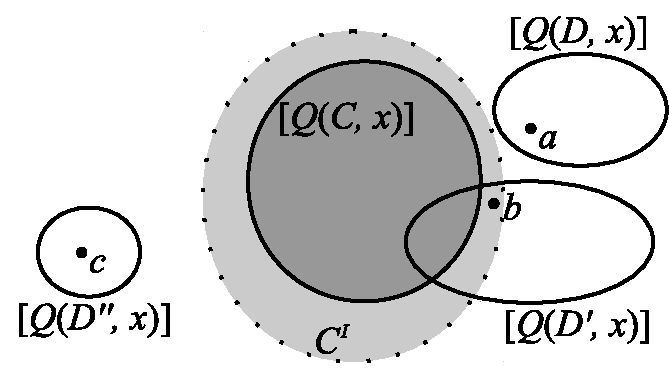
\includegraphics[height=1.4in]{negation}
  \end{center}
  \caption{A schematic illustration of the heuristics used to capture negation
    under the open world assumption. Given a SPARQL graph pattern $Q(\cdot, x)$,
    $[Q(\cdot, x)]$ denotes here the set of individuals that would match variable
    $x$ in the RDF repository at hand. $D''$ is a concept which is declared to
    be disjoint with $C$ in the RDF repository.\label{fig:negation}}
\end{figure}

To compare these three alternative definitions of $Q(\neg C, \mbox{\tt ?x})$,
we may refer to the diagram in Figure~\ref{fig:negation}. We wish to estimate
the actual extent of $(\neg C)^\mathcal{I}$. Clearly, $Q(\neg C, \mbox{\tt ?x})$
(in dark grey) underestimates the real extent of $C^\mathcal{I}$ (in light gray).
Therefore, we may say that Equation~\ref{eq:neg-as-failure} overestimates
the real extent of $(\neg C)^\mathcal{I}$,
in the sense that it will regard as instances of $\neg C$ all individuals $a$
for which ``$a \mbox{\tt\ a } C$'' is not found in the RDF repository.

Now, if $b$ is such that ``$b \mbox{\tt\ a } C$'' is not known, but ``$b \mbox{\tt\ a } D'$''
is known for some class $D'$ and some instances of $D$ are known to be also
instances of $C$, then it might well be that $b$ is an instance of $C$ as well,
although we do not know. If, however $a$ is such that ``$a \mbox{\tt\ a } C$''
is not known, but ``$b \mbox{\tt\ a } D$'' is known for some class $D$ but
no instance of $D$ is known that is also an instance of $C$, then we are more
likely to believe that $a$ is not an instance of $C$.
Therefore Equation~\ref{eq:approx-open-world-negation} regards as instances of $\neg C$
fewer individuals, those for which it is highly likely that they do not belong
in $C$. It might still overestimate the extent of $(\neg C)^\mathcal{I}$, but much less
than Equation~\ref{eq:neg-as-failure}. In fact, it might even underestimate it,
as far as we know.

On the other hand, it is certain that Equation~\ref{eq:negation-with-disjointWith}
will underestimate $(\neg C)^\mathcal{I}$, to the point that it will equate it
with the empty set if no triple of the form ``$D''$ \texttt{owl:disjointWith} $C$''
is declared in the RDF repository. Furthermore, it might well be that an individual
is an instance of $\neg C$ even though it is not an instance of a class disjoint with $C$!

To sum up, Equation~\ref{eq:neg-as-failure} is too optimistic,
Equation~\ref{eq:negation-with-disjointWith} too pessimistic, and
Equation~\ref{eq:approx-open-world-negation} somewhere in the middle.
Following the old adage ``virtue stands in the middle'', adopting
Equation~\ref{eq:approx-open-world-negation} looks like a sensible choice.

\item Existential restriction: the general form is
  \begin{equation}\label{eq:existential-restriction}
    Q(\exists R.C, \mbox{\tt ?x}, \mbox{\tt ?y}) =
      Q(R, \mbox{\tt ?x}, \mbox{\tt ?z1})\ Q(C, \mbox{\tt ?z1}, \mbox{\tt ?z2}),
  \end{equation}
  where \texttt{?z1} and \texttt{?z2} are variables that do not occur anywhere else in the query;
  if $C$ is an extensional concept (\textsf{ObjectOneOf}), Equation~\ref{eq:existential-restriction}
  may be simplified into
  \begin{equation}\label{eq:existential-restriction-extensional}
    Q(\exists R.C, \mbox{\tt ?x}, \mbox{\tt ?y}) =
      \mbox{\tt \{\ } Q(R, \mbox{\tt ?x}, \mbox{\tt ?z1})\ 
      \mbox{\tt FILTER ( ?z1 IN ( } a_1,\ \ldots,\ a_n \mbox{\tt\ ) ) \}.},
  \end{equation}
  while for existential restriction with a nominal (\textsf{ObjectHasValue}),
  Equation~\ref{eq:existential-restriction} reduces to
  \begin{equation}\label{eq:existential-restriction-nominal}
    Q(\exists R.\{a\}, \mbox{\tt ?x}, \mbox{\tt ?y}) = Q(R, \mbox{\tt ?x}, a).
  \end{equation}
  Finally, for the local reflexivity existential restriction (\textsf{ObjectHasSelf}), we have, simply,
  \begin{equation}\label{eq:local-reflexivity-existential-restriction}
    Q(\exists R.\mathsf{Self}, \mbox{\tt ?x}, \mbox{\tt ?y}) =
      Q(R, \mbox{\tt ?x}, \mbox{\tt ?x}).
  \end{equation}

\item Value restriction: 
  B\"uhmann and Lehmann propose
  \begin{equation}
    Q(\forall R.C, \mbox{\tt ?x}, \mbox{\tt ?y}) =
    \begin{minipage}[t]{5in}
      \begin{tabbing}
        \quad\=\quad\=\quad\=\kill
        \{\>$Q(R, \mbox{\tt ?x}, \mbox{\tt ?z0})$\\
        \>\{\>\texttt{SELECT ?x (count(DISTINCT ?z1) AS ?cnt1)}\\
        \>\>\texttt{WHERE \{}\\
        \>\>\>$Q(R, \mbox{\tt ?x}, \mbox{\tt ?z1})$\\
        \>\>\>$Q(C, \mbox{\tt ?z1}, \mbox{\tt ?z2})$\\
        \>\>\} \texttt{GROUP BY ?x}\\
        \>\}\\
        \>\{\>\texttt{SELECT ?x (count(DISTINCT ?z3) AS ?cnt2)}\\
        \>\>\texttt{WHERE \{}\\
        \>\>\>$Q(R, \mbox{\tt ?x}, \mbox{\tt ?z3})$\\
        \>\>\} \texttt{GROUP BY ?x}\\
        \>\}\\
        \>\texttt{FILTER ( ?cnt1 = ?cnt2 )}\\
        \texttt{\} .}
      \end{tabbing}
    \end{minipage}
  \end{equation}
  where \texttt{?z0}, \texttt{?z1}, \texttt{?z2}, \texttt{?z3}, \texttt{?cnt1}, and \texttt{?cnt2}
  are variables that do not occur anywhere else in the query.
  An alternative, more compact way to express the same graph pattern without resorting to counts
  would be
  \begin{equation}
    Q(\forall R.C, \mbox{\tt ?x}, \mbox{\tt ?y}) =
    \begin{minipage}[t]{5in}
      \begin{tabbing}
        \quad\=\quad\=\quad\=\kill
        \{\>$Q(R, \mbox{\tt ?x}, \mbox{\tt ?z0})$\\
        \>\texttt{FILTER NOT EXISTS \{}\\
        \>\>$Q(R, \mbox{\tt ?x}, \mbox{\tt ?z1})$\\
        \>\>\texttt{FILTER NOT EXISTS \{}\\
        \>\>\>$Q(C, \mbox{\tt ?z1}, \mbox{\tt ?z2})$\\
        \>\>\}\\
        \>\}\\
        \texttt{\} .}
      \end{tabbing}
    \end{minipage}
  \end{equation}
  with, once again, \texttt{?z0}, \texttt{?z1}, and \texttt{?z2} three new, unused variables.
  Choosing to use either form should be based on their comparative performance.
  Notice that, for the particular case where $C = \{a_1, \ldots, a_n\}$,
  this query might be replaced by
  \begin{equation}
    Q(\forall R.\{a_1, \ldots, a_n\}, \mbox{\tt ?x}, \mbox{\tt ?y}) =
    \begin{minipage}[t]{5in}
      \begin{tabbing}
        \quad\=\quad\=\quad\=\kill
        \{\>$Q(R, \mbox{\tt ?x}, \mbox{\tt ?z0})$\\
        \>\texttt{FILTER NOT EXISTS \{}\\
        \>\>$Q(R, \mbox{\tt ?x}, \mbox{\tt ?z1})$\\
        \>\>\texttt{FILTER ( ?z1 NOT IN (} $a_1, \ldots, a_n$ \texttt{) )}\\
        \>\}\\
        \texttt{\} .}
      \end{tabbing}
    \end{minipage}
  \end{equation}
  which probably leads to a faster execution, and similarly for $C = \{d_1, \ldots, d_n\}$.

\item Number restrictions:
  B\"uhmann and Lehmann propose, for the qualified number restrictions,
  \begin{equation}\label{eq:qualified-number-restriction}
    Q(\Theta nR.C, \mbox{\tt ?x}, \mbox{\tt ?y}) =
    \begin{minipage}[t]{5in}
      \begin{tabbing}
        \quad\=\quad\=\quad\=\kill
        \{\>$Q(R, \mbox{\tt ?x}, \mbox{\tt ?z0})$\\
        \>\{\>\texttt{SELECT ?x}\\
        \>\>\texttt{WHERE \{}\\
        \>\>\>$Q(R, \mbox{\tt ?x}, \mbox{\tt ?z1})$\\
        \>\>\>$Q(C, \mbox{\tt ?z1}, \mbox{\tt ?z2})$\\
        \>\>\}\\
        \>\>\texttt{GROUP BY ?x}\\
        \>\>\texttt{HAVING ( count(DISTINCT ?z1)} $\Theta$ $n$ \texttt{\ )}\\
        \>\texttt{\}}\\
        \texttt{\} .}
      \end{tabbing}
    \end{minipage}
  \end{equation}
  where \texttt{?z0}, \texttt{?z1}, and \texttt{?z1} are fresh variables
  that do not occur anywhere else in the query and $\Theta \in \{ \leq, =, \geq \}$.
  For an unqualified number restriction, Equation~\ref{eq:qualified-number-restriction} becomes
  \begin{equation}\label{eq:unqualified-number-restriction}
    Q(\Theta nR.\top, \mbox{\tt ?x}, \mbox{\tt ?y}) =
    \begin{minipage}[t]{5in}
      \begin{tabbing}
        \quad\=\quad\=\quad\=\kill
        \{\>$Q(R, \mbox{\tt ?x}, \mbox{\tt ?z0})$\\
        \>\{\>\texttt{SELECT ?x WHERE \{ } $Q(R, \mbox{\tt ?x}, \mbox{\tt ?z1})$ \}\\
        \>\>\texttt{GROUP BY ?x}\\
        \>\>\texttt{HAVING ( count(DISTINCT ?z1)} $\Theta$ $n$ \texttt{\ )}\\
        \>\texttt{\}}\\
        \texttt{\} .}
      \end{tabbing}
    \end{minipage}
  \end{equation}
  These graph patterns, however, break down when the \texttt{?x} variable is replaced
  by a named individual $a$ (an RDF \emph{resource}), as in an \texttt{ASK} query
  to check the membership of $a$ in $\Theta nR.C$. In those cases, they have to be
  replaced by
  \begin{equation}
    Q(\Theta nR.C, a, \mbox{\tt ?y}) =
    \begin{minipage}[t]{5in}
      \begin{tabbing}
        \quad\=\quad\=\quad\=\kill
        \{\>\texttt{SELECT ?z0 WHERE \{}\\
        \>\>\texttt{BIND (} $a$ \texttt{AS ?z0 )}\\
        \>\>$Q(R, \mbox{\tt ?z0}, \mbox{\tt ?z1})$\\
        \>\>$Q(C, \mbox{\tt ?z1}, \mbox{\tt ?z2})$\\
        \>\}\\
        \>\texttt{GROUP BY ?z0}\\
        \>\texttt{HAVING ( count(DISTINCT ?z1)} $\Theta$ $n$ \texttt{\ )}\\
        \texttt{\} .}
      \end{tabbing}
    \end{minipage}
  \end{equation}
  and
  \begin{equation}
    Q(\Theta nR.\top, a, \mbox{\tt ?y}) =
    \begin{minipage}[t]{5in}
      \begin{tabbing}
        \quad\=\quad\=\quad\=\kill
        \{\>\texttt{SELECT ?z0 WHERE \{}\\
        \>\>\texttt{BIND (} $a$ \texttt{AS ?z0 )}\\
        \>\>$Q(R, \mbox{\tt ?z0}, \mbox{\tt ?z1})$\\
        \>\}\\
        \>\texttt{GROUP BY ?z0}\\
        \>\texttt{HAVING ( count(DISTINCT ?z1)} $\Theta$ $n$ \texttt{\ )}\\
        \texttt{\} .}
      \end{tabbing}
    \end{minipage}
  \end{equation}
  respectively.
%{
%  SELECT ?x WHERE {
%     BIND (:The_Jackson_5 AS ?x)
%     ?x dbo:genre ?y .
%  }
%  GROUP BY ?x
%  HAVING ( count(DISTINCT ?y) > 3 )
%}


\end{itemize}

\subsection{The Reckoning of Evidence}

Table~\ref{tab:axiom-semantics} provides a reference of the semantics
of the 32 axiom types of OWL~2. We will take those semantics as a starting point to define,
for each axiom type, which facts recorded in the RDF triple store are to be taken as
supporting evidence, or \emph{confirmations} of the axiom and which facts are to be
construed as refuting evidence, or \emph{counterexamples}, based on the principles
laid out in Section~\ref{epistemology}.
How such positive and negative evidence should be used to evaluate an axiom
will then make the subject of Section~\ref{possibility-theory}.

Quite obviously, resource names occurring in RDF triples will be regarded as
individual names from the point of view of the model-theoretic semantics taken as
a basis for defining evidence. For the sake of clarity, we will make the explicit
assumption that an RDF resource name (= individual name) is mapped by the interpretation
function $\mathcal{I}$ to exactly one element of the interpretation domain $\Delta^\mathcal{I}$
(this follows trivially from the fact that $\mathcal{I}$ is a function);
however, the same element of $\Delta^\mathcal{I}$ may be referred to by more than one
RDF resource name and any two resource names may potentially refer to the same element.
To be even more explicit, synonyms may exist in an RDF triple store, above and beyond
those that are stipulated by \textsf{owl:sameAs} and other equivalent properties.
This assumption reflects indeed what is the actual state of affairs in the LOD cloud.
An immediate consequence of it is that, given two individual names $a$ and $b$,
$a \neq b$ (i.e., $a$ and $b$ are \emph{syntactically} different) is not sufficient,
by itself, to deduce $a^\mathcal{I} \neq b^\mathcal{I}$, or, equivalently, $a \not\doteq b$
(i.e., $a$ and $b$ do not refer to the same entity).

\begin{table}
\caption{The model-theoretic semantics of the axiom types of the Web ontology
language OWL~2. The first column gives the functional-style OWL syntax of the
axiom, the second column its more compact $\mathcal{SHOIQ}$ description logic syntax,
and the last column shows the semantics of the axiom, for all $x$, $y$, and $z$.\label{tab:axiom-semantics}}
\begin{center}\small
\begin{tabular}{|l|l|l|}
\hline
  OWL~2 (functional-style) & DL Syntax & Semantics \\
\hline &&\\[-0.95em]\hline
  $\mathsf{SubClassOf}(C\ D)$ & $C \sqsubseteq D$  & $C^\mathcal{I} \subseteq D^\mathcal{I}$ \\
  $\mathsf{EquivalentClasses}(C_1\ \ldots\ C_n)$ & $C_i \equiv C_j$, $i,j \in \{1, \ldots n\}$ & 
    $C_i^\mathcal{I} = C_j^\mathcal{I}$, $i,j \in \{1, \ldots n\}$ \\
  $\mathsf{DisjointClasses}(C_1\ \ldots\ C_n)$ & $\mathsf{Dis}(C_1, \ldots, C_n)$ &
    $C_i^\mathcal{I} \cap C_j^\mathcal{I} = \emptyset$, $i,j \in \{1, \ldots n\}$, $i\neq j$  \\
  $\mathsf{DisjointUnion}(C\ C_1\ \ldots\ C_n)$ & $C = C_1 \sqcup \ldots \sqcup C_n$, and &
    $C^\mathcal{I} = C_1^\mathcal{I} \cup \ldots \cup C_n^\mathcal{I}$, and \\
  & $\mathsf{Dis}(C_1, \ldots, C_n)$ &
    $C_i^\mathcal{I} \cap C_j^\mathcal{I} = \emptyset$, $i,j \in \{1, \ldots n\}$, $i\neq j$  \\
\hline
  $\mathsf{SubObjectPropertyOf}(S, R)$ & $S \sqsubseteq R$ & $S^\mathcal{I} \subseteq R^\mathcal{I}$ \\
  $\mathsf{SubObjectPropertyOf}(w, R)$, with & $S_1\ldots S_n \sqsubseteq R$ &
    $S_1^\mathcal{I} \circ \ldots \circ S_n^\mathcal{I} \subseteq R^\mathcal{I}$,
    i.e., $\forall y_0, \ldots, y_n$, \\
  \quad$w = \mathsf{ObjectPropertyChain}(S_1\ \ldots\ S_n)$ & &
    $\langle y_0, y_1\rangle \in S_1^\mathcal{I} \land \ldots \land
    \langle y_{n-1}, y_n\rangle \in S_n^\mathcal{I}$ \\
  & & $\Rightarrow \langle y_0, y_n\rangle \in R^\mathcal{I}$ \\
  $\mathsf{EquivalentObjectProperties}(R_1\ \ldots\ R_n)$ & $R_i \equiv R_j$, $i,j \in \{1, \ldots n\}$ & 
    $R_i^\mathcal{I} = R_j^\mathcal{I}$, $i,j \in \{1, \ldots n\}$ \\
  $\mathsf{DisjointObjectProperties}(R_1\ \ldots\ R_n)$ & $\mathsf{Dis}(R_1, \ldots, R_n)$ &
    $R_i^\mathcal{I} \cap R_j^\mathcal{I} = \emptyset$, $i,j \in \{1, \ldots n\}$, $i\neq j$ \\
  $\mathsf{ObjectPropertyDomain}(R\ C)$ & $\geq 1 R \sqsubseteq C$ &
    $\langle x, y\rangle \in R^\mathcal{I} \Rightarrow x\in C^\mathcal{I}$ \\
  $\mathsf{ObjectPropertyRange}(R\ C)$ & $\top \sqsubseteq \forall R.C$ & 
    $\langle x, y\rangle \in R^\mathcal{I} \Rightarrow y\in C^\mathcal{I}$ \\
  $\mathsf{InverseObjectProperties}(S\ R)$ & $S \equiv R^-$ &
    $S^\mathcal{I} = \{\langle y, x \rangle \mid \langle x, y \rangle \in R^\mathcal{I} \}$ \\
  $\mathsf{FunctionalObjectProperty}(R)$ & $\mathsf{Fun}(R)$ &
    $\langle x, y\rangle \in R^\mathcal{I} \land \langle x, z\rangle \in R^\mathcal{I}
    \Rightarrow y = z$ \\
  $\mathsf{InverseFunctionalObjectProperty}(R)$ & $\mathsf{Fun}(R^-)$ &
    $\langle x, y\rangle \in R^\mathcal{I} \land \langle z, y\rangle \in R^\mathcal{I}
    \Rightarrow x = z$ \\
  $\mathsf{ReflexiveObjectProperty}(R)$ & $\mathsf{Ref}(R)$ & $\langle x, x\rangle \in R^\mathcal{I}$ \\
  $\mathsf{IrreflexiveObjectProperty}(R)$ & $\mathsf{Irr}(R)$ & $\langle x, x\rangle \notin R^\mathcal{I}$ \\
  $\mathsf{SymmetricObjectProperty}(R)$ & $\mathsf{Sym}(R)$ &
    $\langle x, y\rangle \in R^\mathcal{I} \Rightarrow \langle y, x\rangle \in R^\mathcal{I}$ \\
  $\mathsf{AsymmetricObjectProperty}(R)$ & $\mathsf{Asy}(R)$ &
    $\langle x, y\rangle \in R^\mathcal{I} \Rightarrow \langle y, x\rangle \notin R^\mathcal{I}$ \\
  $\mathsf{TransitiveObjectProperty}(R)$ & $\mathsf{Tra}(R)$ & 
    $\langle x, y\rangle \in R^\mathcal{I} \land \langle y, z\rangle \in R^\mathcal{I} \Rightarrow
    \langle x, z\rangle \in R^\mathcal{I}$ \\
\hline
  $\mathsf{SubDataPropertyOf}(S, R)$ & $S \sqsubseteq R$ & $S^\mathcal{I} \subseteq R^\mathcal{I}$ \\
  $\mathsf{EquivalentDataProperties}(R_1\ \ldots\ R_n)$ & $R_i \equiv R_j$, $i,j \in \{1, \ldots n\}$ & 
    $R_i^\mathcal{I} = R_j^\mathcal{I}$, $i,j \in \{1, \ldots n\}$ \\
  $\mathsf{DisjointDataProperties}(R_1\ \ldots\ R_n)$ & $\mathsf{Dis}(R_1, \ldots, R_n)$ &
    $R_i^\mathcal{I} \cap R_j^\mathcal{I} = \emptyset$, $i,j \in \{1, \ldots n\}$, $i\neq j$ \\
  $\mathsf{DataPropertyDomain}(R\ C)$ & $\geq 1 R \sqsubseteq C$ &
    $\langle x, y\rangle \in R^\mathcal{I} \Rightarrow x\in C^\mathcal{I}$ \\
  $\mathsf{DataPropertyRange}(R\ D)$ & $\top \sqsubseteq \forall R.D$ & 
    $\langle x, y\rangle \in R^\mathcal{I} \Rightarrow y\in D^\mathcal{I}$ \\
  $\mathsf{FunctionalDataProperty}(R)$ & $\mathsf{Fun}(R)$ &
    $\langle x, y\rangle \in R^\mathcal{I} \land \langle x, z\rangle \in R^\mathcal{I}
    \Rightarrow y = z$ \\
\hline
  $\mathsf{DatatypeDefinition}(T\ D)$ & $T \equiv D$ & $T^\mathcal{I} = D^\mathcal{I}$ \\
\hline
  $\mathsf{HasKey}(C\ (R_1\ \ldots\ R_n)\ (S_1\ \ldots\ S_m))$ & n/a &
    $a, b\in C^\mathcal{I}$\quad$a, a_i, b, b_i$ named individuals \\
  \quad with $R_i$ object properties & & $\land \langle a, a_i\rangle \in R_i^\mathcal{I}
       \land \langle b, b_i\rangle \in R_i^\mathcal{I}$ \\
  \quad and $S_i$ data properties & & $\land \langle a, d_i\rangle \in S_i^\mathcal{I}
       \land \langle b, e_i\rangle \in S_i^\mathcal{I} \Rightarrow a = b$ \\
\hline
  $\mathsf{SameIndividual}(a_1\ \ldots\ a_n)$ & $a_i \doteq a_j$, $i,j\in\{1, \ldots, n\}$ &
    $a_i^\mathcal{I} = a_j^\mathcal{I}$, $i,j \in \{1, \ldots n\}$ \\
  $\textsf{DifferentIndividuals}(a_1\ \ldots\ a_n)$ & $a_i \not\doteq a_j$, $i,j\in\{1, \ldots, n\}$, $i\neq j$ &
    $a_i^\mathcal{I} \neq a_j^\mathcal{I}$, $i,j \in \{1, \ldots n\}$, $i\neq j$ \\
  $\mathsf{ClassAssertion}(C\ a)$ & $C(a)$ & $a^\mathcal{I} \in C^\mathcal{I}$ \\
  $\mathsf{ObjectPropertyAssertion}(R\ a\ b)$ & $R(a, b)$ &
    $\langle a^\mathcal{I}, b^\mathcal{I}\rangle \in R^\mathcal{I}$ \\
  $\mathsf{NegativeObjectPropertyAssertion}(R\ a\ b)$ & $\neg R(a, b)$ &
    $\langle a^\mathcal{I}, b^\mathcal{I}\rangle \notin R^\mathcal{I}$ \\
  $\mathsf{DataPropertyAssertion}(R\ a\ d)$ & $R(a, d)$ &
    $\langle a^\mathcal{I}, d^\mathcal{I}\rangle \in R^\mathcal{I}$ \\
  $\mathsf{NegativeDataPropertyAssertion}(R\ a\ d)$ & $\neg R(a, d)$  &
    $\langle a^\mathcal{I}, d^\mathcal{I}\rangle \notin R^\mathcal{I}$ \\
\hline
\end{tabular}
\end{center}
\end{table}

\subsubsection{Assertions}

The axioms types in the last section of Table~\ref{tab:axiom-semantics} are
assertions involving named individuals or literals.
In particular, we refer here to
\textsf{ClassAssertion}, \textsf{ObjectPropertyAssertion},
\textsf{NegativeObjectPropertyAssertion}, \textsf{DataPropertyAssertion}, and
\textsf{NegativeDataPropertyAssertion}.

These may be further divided into \emph{positive} and \emph{negative} assertions.
Positive assertions are the easiest to check.

TO DO: SHOW HOW.

\subsubsection{Subsumption Axioms}

We can group together all axiom whose semantics may be stated in terms of set inclusion.
This is clearly the case for \textsf{SubClassOf}, \textsf{SubObjectPropertyOf}, and \textsf{SubDataPropertyOf},
but also for \textsf{ObjectPropertyDomain}, \textsf{ObjectPropertyRange},
\textsf{SymmetricObjectProperty}, \textsf{AsymmetricObjectProperty}, \textsf{TransitiveObjectProperty},
\textsf{DataPropertyDomain}, and \textsf{DataPropertyRange}, because an implication of set
membership can be transformed into a set inclusion: for instance,
$\langle x, y\rangle \in R^\mathcal{I} \Rightarrow x\in C^\mathcal{I}$ may be restated as
$\mathrm{Proj}_1(R^\mathcal{I}) \subseteq C^\mathcal{I}$, where $\mathrm{Proj}_i$ is a projection
operator that projects a relation on its $i$th component.
We will call these axioms collectively \emph{subsumption} axioms.

The general principle for subsumption axioms is the following:
let us call $E_\mathrm{sub}$ and $E_\mathrm{super}$ the extensions of the subsumed
expression and the subsuming expression, respectively, as retrieved by the relevant
SPARQL \texttt{SELECT} query. Let us then call $E_\mathrm{sub}^\neg$ and $E_\mathrm{super}^\neg$
the extension of their negated expression. Notice that, in general, this is not the
same as the complement of $E_\mathrm{sub}$ and $E_\mathrm{super}$. In fact,
$E_\mathrm{sub}^\neg \subseteq \overline{E_\mathrm{sub}}$ and
$E_\mathrm{super}^\neg \subseteq \overline{E_\mathrm{super}}$,
because of the open-world hypothesis and the fact that the RDF triple store may not
be complete. Then
\begin{itemize}
\item confirmations are those individual or pairs $x$ such that
  $x \in E_\mathrm{sub}$ and $x \in E_\mathrm{super}$;
\item counterexamples are those individuals or pairs $x$ such that
  $x \in E_\mathrm{sub}$ and $x \in E_\mathrm{super}^\neg$.
\end{itemize}
Notice that an $x \in E_\mathrm{sub}$ such that $x \notin E_\mathrm{super}$
does not contradict a subsumption axiom, because it might well be the case
that the assertion $x \in E_\mathrm{super}$ is just missing from the ABox.
Likewise, an $x \in E_\mathrm{super}^\neg$ such that $x \in E_\mathrm{sub}^\neg$
will not be treated as a confirmation, based on our choice to regard as
evidence in favor of a hypothesis only selective confirmations.

The above general principle may be translated into specific SPARQL queries
that count the confirmations and the exceptions. For example, the two queries
to test an axiom of the form $\mathsf{SubClassOf}(C\ D)$ are
\begin{equation}
  \begin{minipage}[c]{5in}
    \begin{tabbing}
      \quad\=\quad\=\quad\=\kill
      \texttt{SELECT (count(DISTINCT ?x) AS ?numConfirmations) WHERE} \{\\
      \>$Q(C, \mbox{\tt ?x}, \mbox{\tt ?y})$\\
      \>$Q(D, \mbox{\tt ?x}, \mbox{\tt ?y})$\\
      \}
    \end{tabbing}
  \end{minipage}
\end{equation}
and
\begin{equation}
  \begin{minipage}[c]{5in}
    \begin{tabbing}
      \quad\=\quad\=\quad\=\kill
      \texttt{SELECT (count(DISTINCT ?x) AS ?numExceptions) WHERE} \{\\
      \>$Q(C, \mbox{\tt ?x}, \mbox{\tt ?y})$\\
      \>$Q(\neg D, \mbox{\tt ?x}, \mbox{\tt ?y})$\\
      \}
    \end{tabbing}
  \end{minipage}
\end{equation}
respectively.


\subsubsection{Equivalence Axioms}

Another important group of axioms consists of those axioms whose semantics may be
stated in terms of equality of set equality. This is the case for
\textsf{EquivalentClasses}, \textsf{EquivalentObjectProperties},
\textsf{InverseObjectProperties}, \textsf{ReflexiveObjectProperties},
\textsf{EquivalentDataProperties}, and \textsf{DatatypeDefinition}.
Let us call $E_\mathrm{lhs}$ and $E_\mathrm{rhs}$ the extensions of the
left-hand side and of the right-hand side of the equivalence. Then, 
\begin{itemize}
\item confirmations are those individual or pairs $x$ such that
  $x \in E_\mathrm{lhs}$ and $x \in E_\mathrm{rhs}$;
\item counterexamples are those individuals or pairs $x$ such that either
  $x \in E_\mathrm{lhs}$ and $x \in E_\mathrm{rhs}^\neg$ or
  $x \in E_\mathrm{lhs}^\neg$ and $x \in E_\mathrm{rhs}$.
\end{itemize}

\subsubsection{Disjointness Axioms}

The fourth group of axiom consists of those axioms whose semantics may be stated
in terms of set disjunction. These include
\textsf{DisjointClasses}, \textsf{DisjointObjectProperties},
\textsf{IrreflexiveObjectProperty}, and \textsf{DisjointDataProperties}.
Given $E_\mathrm{lhs}$ and $E_\mathrm{rhs}$, the extensions of two
disjoint concepts or relations, 
\begin{itemize}
\item confirmations are those individual or pairs $x$ such that
  either $x \in E_\mathrm{lhs}$ and $x \in E_\mathrm{rhs}^\neg$ or
  $x \in E_\mathrm{lhs}^\neg$ and $x \in E_\mathrm{rhs}$;
\item counterexamples are those individuals or pairs $x$ such that
  $x \in E_\mathrm{lhs}$ and $x \in E_\mathrm{rhs}$.
\end{itemize}
The attentive reader will have noticed that confirmations here are the same
as counterexamples for Equivalence axioms and \emph{vice versa}, counterexamples
here are the same as confirmations for Equivalence Axioms.

A particular case is  \textsf{DisjointUnion}, whose semantics is expressed
both in terms of equivalence and in terms of set disjunctions.

\paragraph{Related Work}

Disjointness axioms have been the object of learning using several different
approaches proposed in the literature:
\begin{itemize}
  \item Classifiers are used by the \href{http://ontoware/projects/leda}{LeDA}
    tool~\cite{VoelkerVrandecicSureHotho2007,MeilickeVoelkerStuckenschmidt2008}%
    ---to be precise, Weka's implementation of Naive Bayes with default parameters,
    which was found to slightly outperform decision trees and SVM.
    The key aspect of this approach is to identify features of OWL classes that can
    lead to a satisfactory performance of the selected classification method.
  \item Statistical schema induction~\cite{VoelkerNiepert2011}, based on
    associative rule mining, is complemented by a simple heuristic
    for introducing disjointness axioms, which assumes classes with non-overlapping
    extensions of more than a hundred individuals to be disjoint.
    Some improvements to this approach have been recently proposed by a team
    of Chinese researchers from Nanjing~\cite{MaGaoWuQi2014}.
  \item Inductive methods based on ILP, namely DL-Learner~\cite{Lehmann2009}.
  \item Inductive methods based on formal concept analysis
    \cite{BaaderGanterSertkayaSattler2007}.
  \item Semantic clarification \cite{Schlobach2005}
    uses the \emph{strong disjointness assumption} \cite{CornetAbuHanna2002},
    which postulates disjointness among sibling classes. However, as rightly
    observed by Fleischhacker and V\"olker~\cite{FleischhackerVoelker2011},
    while such heuristics happens to work quite well for the DBpedia ontology,
    where the majority of sibling concepts are in fact disjoint, in general
    there might be ontologies  where this is not the case. Indeed, in the DBpedia
    ontology itself, the \textsf{dbo:Person} subtree contradicts this assumption.
\end{itemize}
A survey of several of these methods can be found in \cite{FleischhackerVoelker2011}.

\paragraph{Counting Confirmations and Counterexamples}

Given the above definition of a counterexample,
counting the counterexamples of a disjointness axiom $\mathsf{Dis}(C_1, \ldots, C_n)$
is straightforward and may be done with the following conjunctive SPARQL query:
\begin{equation}
  \begin{minipage}[c]{5in}
    \begin{tabbing}
      \quad\=\quad\=\quad\=\kill
      \texttt{SELECT (count(DISTINCT ?x) AS ?numExceptions) WHERE} \{\\
      \>$Q(C_1, \mbox{\tt ?x}, \mbox{\tt ?y})$\\
      \>$\vdots$\\
      \>$Q(C_n, \mbox{\tt ?x}, \mbox{\tt ?y})$\\
      \}
    \end{tabbing}
  \end{minipage}
\end{equation}
On the other hand, counting confirmations is much trickier. Conceptually,
one has to find all the individuals $x$ such that an assertion $C_i(x)$, for some
$i \in \{1, \ldots, n\}$, is in the RDF repository and it is certain that,
for all $j\in \{1, \ldots, n\}$, $j \neq i$, $x^\mathcal{I} \notin C_j^\mathcal{I}$.
The problem, here, is that our best approximation of the open-world negation as a SPARQL query,
given in Equation~\ref{eq:approx-open-world-negation},
is based on some sort of ``heuristic'' disjunction and may be paraphrased as
\begin{equation}
  x^\mathcal{I} \notin C_j^\mathcal{I} \mbox{ if there exists $D$ such that }
  D(x) \mbox{ and } \mathsf{Dis}(C_j, D).
\end{equation}
If we blindly adopt this heuristics, we risk ending up with the paradoxical result
that, if no counterexamples are found, then every $x$ for which $C_j(x)$ is not asserted
in the RDF repository would count as a confirmation. Indeed, a class $D$ such that
$D(x)$ is in the RDF repository and $\mathsf{Dis}(C_j, D)$ would exist: that class
would be $D = C_i$, since, by hypothesis, $C_i$ and $C_j$ would not share any instance.
This would defeat our purpose of approximating as closely as possible the open-world hypothesis.

A workaround we can propose to overcome this difficulty is to treat as confirmations
only those instances that may be said not to belong to class $C_j$ \emph{independently of}
the class $C_i$ to which those instances belong, i.e., by requiring that $D \not\sqsubseteq C_i$.
In other words, an instance $x$ is considered as a confirmation of
$\mathsf{Dis}(C_1, \ldots, C_n)$ if, and only if, $x$ is declared to belong to just
one of the supposedly disjoint classes, $C_i$, and, for all $j \neq i$ there exists
a witness class $D_j$ that is not subsumed by $C_i$, to which $x$ belongs and
which does not share any known instance with $C_j$.

For the sake of simplicity, let us restrict our attention to disjointness axioms
of the form $\mathsf{Dis}(C_1, C_2)$, i.e., involving just two classes. The above
confirmation-counting heuristics may be translated into the following SPARQL query:
\begin{equation}\label{eq:two-class-disjointness-confirmation}
  \begin{minipage}[c]{5in}
    \begin{tabbing}
      \quad\=\quad\=\quad\=\kill
      \texttt{SELECT (count(DISTINCT ?x) AS ?numConfirmations) WHERE} \{\\
      \>\{\\
      \>\>$Q(C_1, \mbox{\tt ?x}, \mbox{\tt ?y})$\\
      \>\>\texttt{?x a ?dc1 .}\\
      \>\>\texttt{?z1 a ?dc1 . }\\
      \>\>$Q(\neg C_1, \mbox{\tt ?z1}, \mbox{\tt ?y1})$\\
      \>\>\texttt{FILTER NOT EXISTS} \{\\
      \>\>\>\texttt{?z2 a ?dc1 . }\\
      \>\>\>$Q(C_2, \mbox{\tt ?z2}, \mbox{\tt ?y2})$\\
      \>\>\}\\
      \>\}\\
      \>\texttt{UNION}\\
      \>\{\\
      \>\>$Q(C_2, \mbox{\tt ?x}, \mbox{\tt ?y})$\\
      \>\>\texttt{?x a ?dc2 .}\\
      \>\>\texttt{?z3 a ?dc2 . }\\
      \>\>$Q(\neg C_2, \mbox{\tt ?z3}, \mbox{\tt ?y3})$\\
      \>\>\texttt{FILTER NOT EXISTS} \{\\
      \>\>\>\texttt{?z4 a ?dc2 . }\\
      \>\>\>$Q(C_1, \mbox{\tt ?z4}, \mbox{\tt ?y4})$\\
      \>\>\}\\
      \>\}\\
      \}
    \end{tabbing}
  \end{minipage}
\end{equation}
To generalize the above query for testing a disjointness axiom involving an arbitrary
number of classes, it will be useful to define a parametric graph pattern
$Q_{\mathsf{Dis}}(E_j \mid E_i, x, y)$, where $E_i$ and $E_j$ are two OWL2 expressions
and $x$ and $y$ are formal parameter which can take up the name of a SPARQL
variable, a resource identifier, or a literal as value, as follows:
\begin{equation}
  Q_{\mathsf{Dis}}(C_j \mid C_i, \mbox{\tt ?x}, \mbox{\tt ?y}) =
  \begin{minipage}[t]{5in}
    \begin{tabbing}
      \quad\=\quad\=\quad\=\kill
      \{\\
      \>\texttt{?x a ?dc .}\\
      \>\texttt{?z1 a ?dc . }\\
      \>$Q(\neg C_i, \mbox{\tt ?z1}, \mbox{\tt ?y1})$\\
      \>\texttt{FILTER NOT EXISTS} \{\\
      \>\>\texttt{?z2 a ?dc . }\\
      \>\>$Q(C_j, \mbox{\tt ?z2}, \mbox{\tt ?y2})$\\
      \>\}\\
      \}
    \end{tabbing}
  \end{minipage}
\end{equation}
where all variables except \texttt{?x} and \texttt{?y} should be replaced by
variable names that do not occur anywhere else in the query in which this
graph pattern is instantiated.

The query in Equation~\ref{eq:two-class-disjointness-confirmation}
may thus be rewritten as
\begin{equation}
  \begin{minipage}[c]{5in}
    \begin{tabbing}
      \quad\=\quad\=\quad\=\kill
      \texttt{SELECT (count(DISTINCT ?x) AS ?numConfirmations) WHERE} \{\\
      \>\{\\
      \>\>$Q(C_1, \mbox{\tt ?x}, \mbox{\tt ?y})$\\
      \>\>$Q_{\mathsf{Dis}}(C_2 \mid C_1, \mbox{\tt ?x}, \mbox{\tt ?y})$\\
      \>\}\\
      \>\texttt{UNION}\\
      \>\{\\
      \>\>$Q(C_2, \mbox{\tt ?x}, \mbox{\tt ?y})$\\
      \>\>$Q_{\mathsf{Dis}}(C_1 \mid C_2, \mbox{\tt ?x}, \mbox{\tt ?y})$\\
      \>\}\\
      \}
    \end{tabbing}
  \end{minipage}
\end{equation}
and the generalized query may be written as an $n$-term disjunctive query as follows:
\begin{equation}
  \begin{minipage}[c]{5in}
    \begin{tabbing}
      \quad\=\quad\=\quad\=\kill
      \texttt{SELECT (count(DISTINCT ?x) AS ?numConfirmations) WHERE} \{\\
      \>\{\\
      \>\>$Q(C_1, \mbox{\tt ?x}, \mbox{\tt ?y})$\\
      \>\>$Q_{\mathsf{Dis}}(C_2 \mid C_1, \mbox{\tt ?x}, \mbox{\tt ?y})$\\
      \>\>$\vdots$\\
      \>\>$Q_{\mathsf{Dis}}(C_n \mid C_1, \mbox{\tt ?x}, \mbox{\tt ?y})$\\
      \>\}\\
      \>\texttt{UNION}\\
      \>\{\\
      \>\>$Q(C_2, \mbox{\tt ?x}, \mbox{\tt ?y})$\\
      \>\>$Q_{\mathsf{Dis}}(C_1 \mid C_2, \mbox{\tt ?x}, \mbox{\tt ?y})$\\
      \>\>$Q_{\mathsf{Dis}}(C_3 \mid C_2, \mbox{\tt ?x}, \mbox{\tt ?y})$\\
      \>\>$\vdots$\\
      \>\>$Q_{\mathsf{Dis}}(C_n \mid C_2, \mbox{\tt ?x}, \mbox{\tt ?y})$\\
      \>\}\\
      \>\texttt{UNION}\\
      \>$\vdots$\\
      \>\texttt{UNION}\\
      \>\{\\
      \>\>$Q(C_n, \mbox{\tt ?x}, \mbox{\tt ?y})$\\
      \>\>$Q_{\mathsf{Dis}}(C_1 \mid C_n, \mbox{\tt ?x}, \mbox{\tt ?y})$\\
      \>\>$\vdots$\\
      \>\>$Q_{\mathsf{Dis}}(C_{n - 1} \mid C_n, \mbox{\tt ?x}, \mbox{\tt ?y})$\\
      \>\}\\
      \}
    \end{tabbing}
  \end{minipage}
\end{equation}
The set of potential falsifiers of axiom $\mathsf{Dis}(C_1, \ldots, C_n)$ is
\[
  \bigcup_{i = 1}^n C_i^\mathcal{I}.
\]


\bigskip

TO DO: GENERALIZE TO THE OTHER DISJOINTNESS AXIOMS

\subsubsection{Identity axioms}

The last class of axiom, comprising what we will call \emph{identity axioms},
is also the most problematic. It contains the three axiom types
\textsf{HasKey}, \textsf{SameIndividual}, and \textsf{DifferentIndividuals}.
To these, we might perhaps add also \textsf{FunctionalObjectProperty},
\textsf{InverseFunctionalObjectProperty}, and \textsf{FunctionalDataProperty},
in which identity plays an important role as well.

Verifying if two distinct resource names refer to the same real-world object,
i.e., if they are synonyms,
is one of the trickiest problems, which is closely linked to defining what is a
legitimate \emph{key} (in the database sense) for an entity.

Essentially, recognizing synonyms and connecting them via the \textsf{owl:sameAs}
property is the central problem to be solved to carry out what different authors
call data interlinking, integration, or alignment. Instance-level equivalences are
nowadays the most widely used means for bridging the gap between different data sets.
It is therefore hardly surprising that a vast literature exists which addresses
this problem.

The problem of discovering ``same" entities in different data sets, known as
the \emph{record linkage problem}, is quite well known in database community,
where a large body of literature exists on the topic \cite{Winkler2006}.
The Semantic Web community has built upon those results and proposed its set
os solutions~\cite{EuzenatShvaiko2007}.

Automatic tools for the discovery of equivalent entities
in the Web of data exploit, similarly to ontology matching or record linkage
tools, lexical and/or structural similarities between the entities of different
data sets.
The LinksB2N algorithm~\cite{IseleJentzschBizer2010,SalvadoresEtAl2009} is based
on the idea that the unique combination of RDF predicates associated with RDF
resources is what defines their identity. It should be noted that this idea
is strictly related to the idea of a key, discussed below.
The \href{http://wifo5-03.informatik.uni-mannheim.de/bizer/silk/}{Silk framework}~%
\cite{IseleJentzschBizer2010},
a tool for discovering relationships between data items within different Linked Data sources,
is much more general: it uses a declarative link specification language
to allow the user to specify which types of RDF links should be discovered
and which conditions data items must fulfill in order to be interlinked.
These link conditions may combine various similarity metrics and can take
the graph around a data item into account. Silk accesses the data sources
that should be interlinked via the SPARQL protocol. 
In addition, the new ActiveGenLink algorithm~\cite{IseleBizer2013}
combines genetic programming and active learning to generate expressive linkage
rules interactively.

At first sight, identity would seem to be utterly simple and unproblematic:
everything is identical to itself and
nothing is ever identical to anything else except itself.
The classical theory of identity defines identity (represented by $=$)
with the help of two principles:
\begin{enumerate}
\item $x = x$ (Reflexivity),
\item $x = y \Rightarrow (E(x) \Leftrightarrow E(y))$ (Indiscernibility of Identicals),
\end{enumerate}
where $x$ and $y$ are individuals and $E(x)$ is any statement about $x$.
The principle of indiscernibility of identicals may be reformulated,
in the context of description logics, as:
\begin{enumerate}
\item[2a.] $a \doteq b \Rightarrow (C(a) \Leftrightarrow C(b))$,
\item[2b.] $a \doteq b \Rightarrow (R(a, x) \Leftrightarrow R(b, x)) \land (R(x, a) \Leftrightarrow R(x, b))$,
\end{enumerate}
for all concept $C$ and relation $R$.
In other words, we may establish the following sufficient conditions for distinctness:
given two individual names $a$ and $b$, $a \not\doteq b$ if at least one of the following holds
for some class $C$ or property $R$ and some individual $x$:
\begin{enumerate}
\item $a \in E_C$ and $b \in E_C^\neg$;
\item $b \in E_C$ and $a \in E_C^\neg$;
\item $\langle a, x\rangle \in E_R$ and $\langle b, x\rangle \in E_R^\neg$;
\item $\langle b, x\rangle \in E_R$ and $\langle a, x\rangle \in E_R^\neg$;
\item $\langle x, a\rangle \in E_R$ and $\langle x, b\rangle \in E_R^\neg$;
\item $\langle x, b\rangle \in E_R$ and $\langle x, a\rangle \in E_R^\neg$.
\end{enumerate}
Therefore, it is possible to verify that two individuals are distinct---it suffices
to find a class or property with respect to which the two individuals differ.
On the contrary, one can never conclude that two individual names refer to the same
individual based on the assertions recorded in an ABox, because of the open-world hypothesis.
All identities are bound to be conjectural in nature, except in presence of a key axiom.

A key axiom, specified in OWL~2 by the \textsf{HasKey} keyword, states that
each named instance of a class is uniquely identified by a (data or object) property
or a set of properties---that is, if two named instances of the class coincide
on values for each of the key properties, then these two individuals are the same.
The concept of a \emph{key} derives from database theory. In the entity-relationship
model, a \emph{superkey} is a set of attributes which, taken collectively, uniquely
identify an entity; \emph{candidate keys} are minimal superkeys, in the sense that
they are superkeys for which no proper subset is a superkey. In general, an entity
may have more than one candidate key. A \emph{primary key} for an entity is
the candidate key that is chosen by the database designer as the principal means
of identifying entities within an entity set (i.e., a table in a relational database).
Now, the way the model-theoretic semantics of \textsf{HasKey} is defined in OWL~2
makes it coincide with the notion of a \emph{superkey} in databases. In other words,
a key axiom identifies a \emph{sufficient} set of conditions for two individuals
of a class to refer to the same entity, but not necessarily the smallest such set.

We may therefore use \textsf{HasKey} to provide a sufficient condition for identity
as follows.
Given two individual names $a$ and $b$, $a \doteq b$ if there exists a class $C$
such that all of the following hold:
\begin{enumerate}
\item $C(a)$;
\item $C(b)$;
\item $\mathsf{HasKey}(C\ (R_1\ \ldots\ R_n)\ (S_1\ \ldots\ S_m))$;
\item $\exists x_i : R_i(a, x_i)$ and $R_i(b, x_i)$, for $i = 1, \ldots, n$;
\item $\exists x_j : S_j(a, x_j)$ and $S_j(b, x_j)$, for $j = 1, \ldots, m$.
\end{enumerate}

TO DO : CONCLUDE BY DEFINING EXAMPLES AND COUNTEREXAMPLES
        FOR \textsf{SameIndividual} AND \textsf{DifferentIndividuals}

When it comes to testing a key axiom, we have to turn its semantics the other way aroud
by \emph{modus tollens}:
\begin{itemize}
\item a confirmation of $\mathsf{HasKey}(C\ (R_1\ \ldots\ R_n)\ (S_1\ \ldots\ S_m))$
  consists of two individuals $a$ and $b$ such that at least one of the sufficient
  conditions for the distinctness of $a$ and $b$ ($a \not\doteq b$) given above holds,
  $C(a)$, $C(b)$, and, furthermore,
  there exists a (data or object) property $R \in \{ R_1\ \ldots\ R_n, S_1\ \ldots\ S_m \}$
  such that $R(a, x)$, $R(b, y)$ and $x \not\doteq y$---in other words,
  the key succeeds in distinguishing $a$ and $b$;
\item a counterexample of $\mathsf{HasKey}(C\ (R_1\ \ldots\ R_n)\ (S_1\ \ldots\ S_m))$
  consists of two individuals $a$ and $b$ such that $C(a)$ and $C(b)$,
  and for all $i = 1, \ldots, n$, there exists an individual $c_i$
  such that $R_i(a, c_i)$ and $R_i(b, c_i)$
  and for all $j = 1, \ldots, m$, there exists an individual $d_j$
  such that $S_j(a, d_j)$ and $S_j(b, d_i)$,
  but at least one of the sufficient conditions for the distinctness of $a$ and $b$
  ($a \not\doteq b$) given above holds.
\end{itemize}

TO DO : DEFINE EXAMPLES AND COUNTEREXAMPLES FOR \textsf{FunctionalObjectProperty},
\textsf{InverseFunctionalObjectProperty}, AND \textsf{FunctionalDataProperty}.


\section{Possibilistic Evaluation of Axioms}
\label{possibility-theory}

We propose here two functions for evaluating the possibility and the necessity of
an axiom which try to model the basic intuition behind this process in light of
the discussion provided in Section~\ref{epistemology}.
Of course, alternative proposals are possible and we do not claim that ours is the best or
the only one.

Since any RDF repository is a closed set of facts, but the open-world hypothesis
holds, the knowledge base represented by the RDF repository is incomplete.
Moreover, given the heterogeneous and collaborative character of the linked open data,
some facts in the RDF repository may be erroneous; therefore, there is uncertainty,
although not probabilistic in nature. That is why possibility theory is justified
choice as a framework for describing the knowledge extracted from an RDF repository.

\subsection{Fuzzy Sets and Possibility Theory}

\begin{figure}
  \begin{center}
    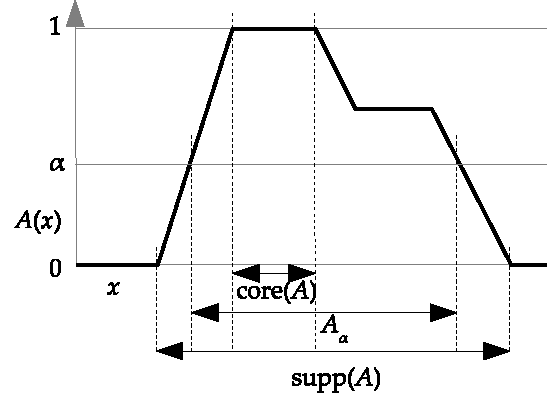
\includegraphics[height=2in]{fuzzyset}
  \end{center}
  \caption{Core, support, and $\alpha$-cuts of a set $A$ of the
    real line.\label{fig:alphacuts}}
\end{figure}

Fuzzy sets \cite{Zadeh1965} are a generalization of classical (crisp) sets obtained by
replacing the characteristic function of a set $A$, $\chi_A$,
which takes up values in $\{0, 1\}$ ($\chi_A(x) = 1$ iff $x \in A$,
$\chi_A(x) = 0$ otherwise) with a \emph{membership function}
$\mu_A$, which can take up any value in $[0, 1]$. The value
$\mu_A(x)$ or, more simply, $A(x)$ is the membership degree of element $x$ in $A$, i.e.,
the degree to which $x$ belongs in $A$.

A fuzzy set is completely defined by its membership
function. Therefore, it is useful to define a few terms describing
various features of this function, summarized in Figure~\ref{fig:alphacuts}.
Given a fuzzy set $A$, its \emph{core} is the (conventional) set
of all elements $x$ such that $A(x) = 1$; its \emph{support}, $\Sup(A)$,
is the set of all $x$ such that $A(x) > 0$.
A fuzzy set is \emph{normal} if its core is nonempty.
The set of all elements $x$ of $A$ such that $A(x)\geq\alpha$,
for a given $\alpha\in(0, 1]$, is called the $\alpha$-cut of $A$,
denoted $A_{\alpha}$.

\subsubsection{Operations on Fuzzy Sets}

The usual set-theoretic operations of union, intersection, and complement
can be defined as a generalization of their counterparts on classical
sets by introducing two families of operators, called triangular norms
and triangular co-norms.
In practice, it is usual to employ the $\min$ norm
for intersection and the $\max$ co-norm for union.
Given two fuzzy sets $A$ and $B$, and an element $x$,
\begin{eqnarray}
 (A \cup B)(x) &=& \max\{A(x), B(x)\}; \\
 (A \cap B)(x) &=& \min\{A(x), B(x)\}; \\
 \bar A(x) &=& 1 - A(x).
\end{eqnarray}
Finally, given two fuzzy sets $A$ and $B$,
$A \subseteq B$ if and only if, for all element $x$,
$A(x) \leq B(x)$.

% \begin{definition}[Fuzzy Interpretation]
% \label{interpretation}
%   A fuzzy interpretation is an assignment of truth degrees in $[0, 1]$ to all
%   atomic propositions (or atoms, for short) defined in the problem domain.
%   Given a set of atoms $\mathcal{A}$, a fuzzy interpretation is a function
%   $
%     \omega : \mathcal{A} \to [0, 1],
%   $
%   which assigns a truth degree $\omega(p) \in [0, 1]$ to all atoms
%   $p \in \mathcal{A}$.
% \end{definition}
% Note that a fuzzy interpretation is, in all respects, a fuzzy set of atoms.

\subsubsection{Possibility Theory}
\label{PossibilityTheory}

The membership function of a fuzzy set describes the more or less 
possible and mutually exclusive values of one (or more) variable(s).
Such a function can then be seen as a possibility distribution
\cite{Zadeh1978}. Indeed, if $F$ designates the fuzzy set of possible
values of a variable $X$, $\pi_X=\mu_F$ is called the possibility 
distribution associated to $X$. The identity $\mu_F(v)=\pi_X(v)$
means that the membership degree of $v$ to $F$ is equal to the 
possibility degree of $X$ being equal to $v$ when all we know about 
$X$ is that its value is in $F$. A possibility distribution for 
which there exists a completely possible value ($\exists v_0; \pi(v_0) = 1$) 
is said to be \emph{normalized}.

There is a similarity between possibility distribution and probability 
density. However, it must be stressed that if $\pi(v)=1$ it just means that
$v$ is a plausible (normal) situation and therefore should not be excluded.
A degree of possibility
can then be viewed as an upper bound of a degree of probability.
Possibility theory is suitable to represent incomplete knowledge while 
probability is adapted to represent random and observed phenomena. 
We invite the reader to see~\cite{dubois1991} for more informations
about the relationships between fuzzy set, possibility and probability 
degrees.
% In particular, the complete ignorance
% about x is expressed by px(u) = 1, for all u . U, because in this case all
% values u are plausible for x and so it is impossible to exclude any of them.
% Whereas, px(¯u) = 1 for a specific value ¯u and px(u) = 0 otherwise, expresses the
% complete knowledge about x, because in this case only the value ¯u is plausible
% for x.

\begin{definition}[Possibility and Necessity Measures] %~\\
A possibility distribution $\pi$ induces a \emph{possibility
measure}\index{possibility measure} and its dual \emph{necessity
measure}\index{necessity measure}, denoted by $\Pi$ and $N$
respectively. Both measures apply to a crisp set $A$ and are
defined as follows:
\begin{eqnarray}
  \Pi(A) &=& \max_{s\in A} \pi(s); \\
  N(A)   &=& 1 - \Pi(\bar{A}) = \min_{s\in \bar{A}} \{1 - \pi(s)\}.
\end{eqnarray}
\end{definition}

In words, the possibility measure of set $A$ corresponds to the
greatest of the possibilities associated to its elements; conversely,
the necessity measure of $A$ is equivalent to the impossibility of
its complement $\bar{A}$.

A few properties of possibility and necessity measures 
induced by a normalized possibility distribution on a finite universe of
discourse $\Omega$ are the following. For all subsets $A, B\subseteq \Omega$:
\begin{enumerate}
  \item $\Pi(A \cup B) = \max\{\Pi(A), \Pi(B)\}$;
  \item $\Pi(A \cup \bar A) = \max\{\Pi(A), \Pi(\bar A)\}=1$;
  \item $\Pi(\emptyset) = N(\emptyset) = 0$,\quad $\Pi(\Omega) = N(\Omega) = 1$;
  \item $N(A \cap B) = \min\{N(A), N(B)\}$;
  \item $\Pi(A) = 1 - N(\bar{A})$ (duality);
  \item $N(A) \leq \Pi(A)$;
  \item $N(A) > 0$ implies $\Pi(A) = 1$;
  \item $\Pi(A) < 1$ implies $N(A) = 0$.
\end{enumerate}
A consequence of these properties is that $\max\{\Pi(A), \Pi(\bar{A})\} = 1$.
In case of complete ignorance on $A$, $\Pi(A) = \Pi(\bar{A}) = 1$.

\subsection{Possibility and Necessity of an Axiom}

The basic principle for establishing the possibility of a formula $\phi$ should be
that the absence of counterexamples to $\phi$ in the RDF repository means $\Pi([\phi]) = 1$,
i.e., that $\phi$ is completely possible.

In general, we may say that a hypothesis should be regarded as all the more
\emph{necessary} as it is explicitly supported by facts and not contradicted by any fact;
all the more \emph{possible} as it is not contradicted by facts.
In other words, given hypothesis $\phi$, $\Pi(\phi) = 1$ if no counterexamples are found;
as the number of counterexamples increases, $\Pi(\phi) \to 0$ strictly monotonically;
$N(\phi) = 0$ if no confirmations are found; as the number of confirmation increases
and no counterexamples are found, $N(\phi) \to 1$ strictly monotonically.
Notice that a confirmation of $\phi$ is a counterexample of $\neg\phi$
an that a counterexample of $\phi$ is a confirmation of $\neg\phi$.

Popper's definition of the \emph{content} of a theory is the set of its logical consequences.
The \emph{relative content} is the set of logical consequences of the theory
given some background knowledge minus all the logical consequences of the
background knowledge (Cf.~\cite{Popper1972}, Page~49 ff.).

For each axiom type $T$, we define a \emph{basic statement} for $T$ as a minimal
ground formula, whose atomic formulas are of the form $C(a)$ or $R(a, b)$,
where $a$ and $b$, $C$, and $R$ are, respectively, an individual name,
an individual name or a literal, a class name,
and a property name occurring in the given RDF store, instantiating the semantics
of axiom type $T$ and thus capable of falsifying an axiom of type $T$.
For instance, basic statements for \textsf{SubClassOf} axioms (of the form $C \sqsubseteq D$)
are all formulas of the form $C(a) \Rightarrow D(a)$, with $a$, $C$, and $D$,
respectively, an individual name and class names occurring in the given RDF store.
We will denote by $\mathrm{BS}_T$ the set af all basic statements for $T$
and by $\mathrm{BS} = \bigcup_T \mathrm{BS}_T$ the set of all basic statements
for the RDF store at hand.

Since an RDF store contains a finite number of triples, only a finite number of
individual, class, and property names and literals can occur in it. Furthermore, the semantics
of all OWL~2 axiom is expressed by a formula constructed from a finite number of
atomic formulas. Therefore, for all axiom type $T$, $\mathrm{BS}_T$ is finite
and so is $\mathrm{BS}$.

Let $\phi$ be an axiom that we wish to evaluate (i.e., a theory).
We define the \emph{content} of an axiom $\phi$ that we wish to evaluate
as the set of its logical consequences, but we restrict it to basic statements, 
to ensure finiteness and testability:
\begin{equation}\label{eq:content}
  \mathrm{content}(\phi) = \{\psi : \phi \models \psi\} \cap \mathrm{BS}.
\end{equation}
The cardinality of $\mathrm{content}(\phi)$ is finite, because $\mathrm{BS}$ is finite,
and every formula $\psi \in \mathrm{content}(\phi)$ may be tested by means of a
SPARQL \texttt{ASK} query, because it is a basic statement.

Let $B$ be some ``background knowledge'' (a set of accepted axioms, or an existing ontology).
Then we may define the content of $\phi$ relative to $B$ as
\begin{equation}\label{eq:relative-content}
  \mathrm{content}(\phi \mid B) = \{\psi : B \cup \{\phi\} \models \psi \mbox{ and } B \not\models \psi\} \cap \mathrm{BS}
  = \mathrm{content}(B \cup \{\phi\}) \setminus \mathrm{content}(B).
\end{equation}
Now, the \emph{truth content} of $\phi$ relative to $B$ is the subset
of $\mathrm{content}(\phi \mid B)$ which is true and the \emph{falsity content}
of $\phi$ relative to $B$ is the subset of $\mathrm{content}(\phi \mid B)$ which
is false.
For instance, if $\phi = C \sqsubseteq D$, $\mathrm{content}(\phi)$ will include
all the facts of the form $C(x) \Rightarrow D(x)$, where $x$ may be replaced by
any individual in the ABox.

Another related concept is Alain and Fabien's idea of \emph{cognitive cost},
defined as the length of the chain of inferences that is required to come to a
conclusion. This idea was used in the context of human-machine interfaces,
but it can probably be adapted to this problem as well.
TO DO: PROVIDE REFERENCES AND DEVELOP

Let us define $u_\phi = \|\mathrm{content}(\phi)\|$ as the cardinality of the
set of facts that are a consequence of $\phi$, i.e., of its potential falsifiers.
For the axiom $C \sqsubseteq D$, it would be $u_{C \sqsubseteq D} = \|C^\mathcal{I}\|$.
This is like a universe of discourse when all we are interested in is to establish
whether hypothesis $\phi$ should be accepted or rejected.
In a sense, we may regard $u_\phi$ as an index of what Popper calls the \emph{boldness}
of theory $\phi$.

Let then $u_\phi^+$ be the number of confirmations and $u_\phi^-$ the number of counterexamples
that are actually found in the RDF repository.
Notice that $u_\phi^+$ will be at most the cardinality of the truth content of $\phi$,
while $u_\phi^-$ will be at most the cardinality of the falsity content of $\phi$.
A few interesting properties of these three cardinalities are:
\begin{enumerate}
\item $u_\phi^+ + u_\phi^- \leq u_\phi$;
\item $u_\phi^+ = u_{\neg\phi}^-$;
\item $u_\phi^- = u_{\neg\phi}^+$;
\item $u_\phi = u_{\neg\phi}$.
\end{enumerate}

Here are a few postulates, based on our previous discussion, the possibility
and necessity functions should obey:
\begin{enumerate}
\item $\Pi(\phi) = 1$ if $u_\phi^- = 0$;
\item $N(\phi) = 0$ if $u_\phi^- > 0$ or $u_\phi^+ = 0$;
\item let $u_\phi = u_\psi$; then $\Pi(\phi) > \Pi(\psi)$ iff $u_\phi^- < u_\psi^-$;
\item let $u_\phi = u_\psi$; then $N(\phi) > N(\psi)$ iff $u_\phi^+ > u_\psi^+$ and $u_\phi^- = 0$;
\item let $u_\phi = u_\psi = u_\chi$ and let $u_\psi^- < u_\phi^- < u_\chi^-$: then
  \[
    \frac{\Pi(\psi) - \Pi(\phi)}{u_\phi^- - u_\psi^-} > \frac{\Pi(\phi) - \Pi(\chi)}{u_\chi^- - u_\phi^-},
  \]
  i.e., the first counterexamples found to an axiom should determine a sharper decrease
  of the degree to which we regard the axiom as possible than any further counterexamples,
  because these latter will only confirm our suspicions and, therefore, will provide
  less and less information;
\item let $u_\phi = u_\psi = u_\chi$ and $u_\psi^- = u_\phi^- = u_\chi^- = 0$,
  and let $u_\psi^+ < u_\phi^+ < u_\chi^+$: then
  \[
    \frac{N(\phi) - N(\psi)}{u_\phi^+ - u_\psi^+} > \frac{N(\chi) - N(\phi)}{u_\chi^+ - u_\phi^+},
  \]
  i.e., in the absence of counterexamples,
  the first confirmations found to an axiom should determine a sharper increase
  of the degree to which we regard the axiom as necessary than any further confirmations,
  because these latter will only add up to our acceptance and, therefore, will provide
  less and less information.\footnote{Cf.\ Popper in the English version of
  \cite{Popper1935}, \S83, 2nd paragraph:
  ``When trying to appraise the degree of corroboration of a theory
    we may reason somewhat as follows. Its degree of corroboration
    will increase with the number of its corroborating instances.
    Here we usually accord to the first corroborating instances far greater
    importance than to later ones: once a theory is well corroborated,
    further instances raise its degree of corroboration only very little.''};
\end{enumerate}

A definition of $\Pi$ and $N$ which satisfies the above postulates is, for $u_\phi > 0$,
\begin{eqnarray}
  \Pi(\phi) &=& 1 - \sqrt{1 - \left(\frac{u_\phi - u_\phi^-}{u_\phi}\right)^2}; \\
  N(\phi) &=& \sqrt{1 - \left(\frac{u_\phi - u_\phi^+}{u_\phi}\right)^2},\quad
    \mbox{if $\Pi(\phi) = 1$, 0 otherwise.}
\end{eqnarray}
Notice that this is by no means the only possible definition.

Figure~\ref{fig:poss-nec-plots} shows $\Pi(\phi)$ and $N(\phi)$ as a function of
$u_\phi^-$ and $u_\phi^+$, respectively. The two functions describe an arc of
an ellipse between the minor and the major axis.

\begin{figure}
  \begin{center}
    \begin{tabular}{cc}
      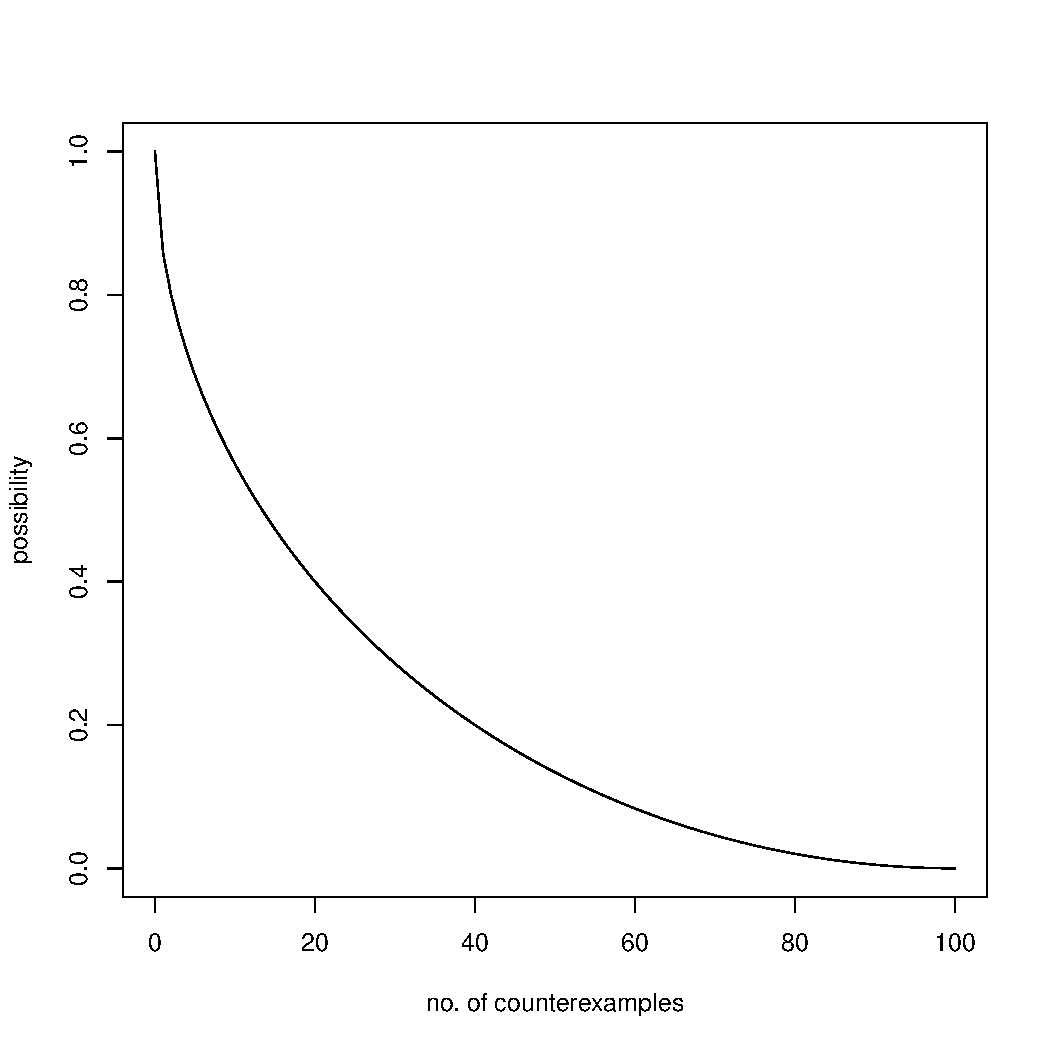
\includegraphics[width=2.5in]{possibility} &
      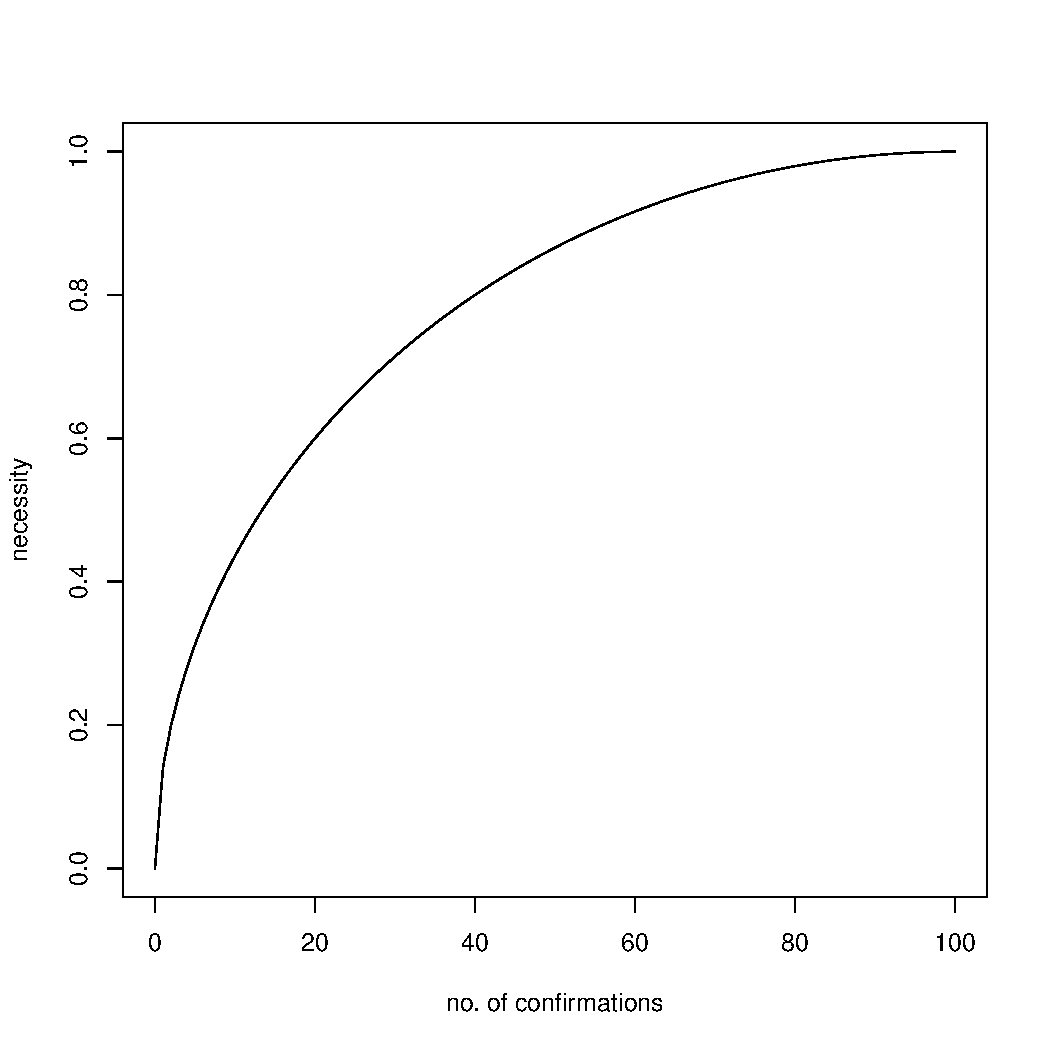
\includegraphics[width=2.5in]{necessity} \\
      (a) & (b)
    \end{tabular}
  \end{center}
  \caption{A plot of $\Pi(\phi)$  as a function of
    $u_\phi^-$ (a) and of $N(\phi)$ as a function of
    $u_\phi^+$ (b) when $u_\phi = 100$.\label{fig:poss-nec-plots}}
\end{figure}

It should be easy tho verify that the above definition satisfies the duality of
possibility and necessity, in that $N(\phi) = 1 - \Pi(\neg\phi)$ and
$\Pi(\phi) = 1 - N(\neg\phi)$.
As a matter of fact, we will seldom be interested in computing the necessity and
possibility degrees of the negation of OWL~2 axioms, for the simple reasons that, in most cases,
the latter are not OWL~2 axioms themselves. For instance, while $C \sqsubseteq D$
is an axiom, $\neg(C \sqsubseteq D) = C \not\sqsubseteq D$ is not.
Notable exceptions are the assertions: \textsf{DifferentIndividuals} is the
negation of \textsf{SameIndividuals}, \textsf{NegativeObjectPropertyAssertion}
is the negation of \textsf{ObjectPropertyAssertion}, and
\textsf{NegativeDataPropertyAssertion} is the negation of \textsf{DataPropertyAssertion}.

The behavior of the first derivative of $\Pi(\phi)$ and $N(\phi)$ is
\[
  \begin{array}{rclcrcl}
    \displaystyle \lim_{u_\phi^-\to0}\frac{d\Pi(\phi)}{du_\phi^-} &=& -\infty, &\quad&
    \left.\frac{d\Pi(\phi)}{du_\phi^-}\right|_{u_\phi} &=& 0, \\
    \displaystyle \lim_{u_\phi^+\to0}\frac{dN(\phi)}{du_\phi^+} &=& +\infty, &\quad&
    \left.\frac{dN(\phi)}{du_\phi^+}\right|_{u_\phi} &=& 0.
  \end{array}
\]
This means that the possibility of $\phi$ decreases very steeply if even a few
counterexamples are found and goes to zero as more and more counterexamples
accumulate. Similarly, even a few confirmations are sufficient to boost the
necessity of $\phi$, but then $N(\phi)$ goes to 1 more and more slowly as
confirmations pile up.

For example, let us assume that we want to calculate the degree of possibility of the axiom
\[
  \mathsf{DisjointObjectProperties}(\mathsf{isFatherOf}, \mathsf{isChildOf}).
\]
In this case, $\phi = \mathsf{Dis}(R, S)$, where $R = \mathsf{isFatherOf}$ and
$S = \mathsf{isChildOf}$.

\textbf{TO DO: DEVELOP THE EXAMPLE}

\subsection{Probabilistic Score of an Axiom}

An alternative to the possibilistic approach we propose to the evaluation of axioms
which has been used in the framework of knowledge base enrichment is based on probability.
For instance, the approach used by B\"uhmann and Lehmann~\cite{BuehmannLehmann2012}
may be regarded essentially as scoring an axiom by an estimate of the probability
that one of its logical consequences is confirmed (or, alternatively, falsified)
by the facts stored in the RDF repository.

This relies on the assumption of a binomial distribution, which applies when an
experiment (here, checking if a logical consequence of a candidate axiom is confirmed
by the facts) is repeated a fixed number of times, each trial having two possible outcomes
(conventionally labeled \emph{success} and \emph{failure}; here, we might call them
\emph{confirmation}, if the observed fact agrees with the candidate axiom,
and \emph{counterexample}, if the observed fact contadicts it),
the probability of success being the same for each observation,
and the observations being statistically independent.

Estimating the probability of confirmation of axiom $\phi$ just by $\hat{p}_\phi = u_\phi^+/u_\phi$
would be too crude and would not take the cardinality of the content of $\phi$
in the RDF repository into account.
The parameter estimation must be carried out by performing a statistical inference.

One of the most basic analyses in statistical inference is to form a confidence interval
for a binomial parameter $p_\phi$ (probability of confirmation of axiom $\phi$), given
a binomial variate $u_\phi^+$ for sample size $u_\phi$ and a sample proportion $\hat{p}_\phi = u_\phi^+/u_\phi$.
Most introductory statistics textbooks use to this end the Wald confidence interval,
based on the asymptotic normality of $\hat{p}_\phi$ and estimating the standard error.
This $(1 - \alpha)$ confidence interval for $p_\phi$ would be
\begin{equation}\label{eq:Wald}
  \hat{p}_\phi \pm z_{\alpha/2}\sqrt{\hat{p}_\phi(1 - \hat{p}_\phi)/u_\phi},
\end{equation}
where $z_c$ denotes the $1 - c$ quantile of the standard normal distribution.

However, the central limit theorem applies poorly to this binomial distribution
with $u_\phi<30$ or where $\hat{p}_\phi$ is close to 0 or 1.
The normal approximation fails totally when $\hat{p}_\phi = 0$ or $\hat{p}_\phi = 1$.
That is why B\"uhmann and Lehmann~\cite{BuehmannLehmann2012} base their probabilistic score
on Agresti and Coull's binomial proportion confidence interval~\cite{AgrestiCoull1998},
an adjustment of the Wald confidence interval which goes: ``Add two successes and two failures
and then use Formula~\ref{eq:Wald}.'' Such adjustment is specific for constructing
95\% confidence intervals.

In fact, Agresti and Coull's suggestion is a simplification of the Wilson score interval
\begin{equation}
  \left(
    \hat{p}_\phi + \frac{z_{\alpha/2}^2}{2u_\phi} \pm
    z_{\alpha/2}\sqrt{\frac{\hat{p}_\phi(1 - \hat{p}_\phi) + \frac{z_{\alpha/2}^2}{4u_\phi}}{u_\phi}}
  \right) / \left(1 + \frac{z_{\alpha/2}^2}{2u_\phi}\right),
\end{equation}
which is an approximate binomial confidence interval obtained by inverting the approximately
normal test that uses the null, rather than the estimated, standard error.
When used to compute the 95\% score interval, this confidence interval
has coverage probabilities close to the nominal confidence level and can be recommended
for use with nearly all sample sizes and parameter values.

A remark about B\"uhmann and Lehmann's approach is in order.
B\"uhmann and Lehmann only look for confirmations of $\phi$, and treat
the absence of a confirmation as a failure in the calculation of the confidence interval.
This is like making an implicit closed-world assumption. In reality, the probability
of finding a confirmation and the probability of finding a counterexample do not add to one,
because there is a non-zero probability of finding neither a confirmation nor a counterexample
for every potential falsifier of an axiom. Their scoring method should thus be
corrected in view of the open-world assumption, for example by using
$\hat{p}^* = u_\phi^+/(u_\phi^+ + u_\phi^-)$ as the sample proportion instead of $\hat{p}$.

However, there is a more fundamental critique to the very idea of computing the likelihood
of axioms based on probabilities. In essence, this idea relies on the assumption
that it is possible to compute the probability that an axiom $\phi$ is true given
some evidence $e$, for example $e$ = ``$\psi \in \mathrm{content}(\phi)$ is in the RDF repository'',
or $e$ = ``$\psi \notin \mathrm{content}(\phi)$ is in the RDF repository'',
or $e$ = ``$\psi \in \mathrm{content}(\phi)$ is not in the RDF repository'', etc.,
which, by Bayes' formula, may be written as
\begin{equation}
  \Pr(\phi \mid e) =
    \frac{\Pr(e \mid \phi)\Pr(\phi)}{\Pr(e \mid \phi)\Pr(\phi) + \Pr(e \mid \neg\phi)\Pr(\neg\phi)}
\end{equation}
However, in order to compute (or estimate) such probability,
one should at least be able to estimate probabilities such as
\begin{itemize}
\item the probability that a fact confirming $\phi$ is added to the repository
  given that $\phi$ holds;
\item the probability that a fact contradicting $\phi$ is added to the repository
  in error, i.e., given that $\phi$ holds;
\item the probability that a fact confirming $\phi$ is added to the repository
  in error, i.e., given that $\phi$ does not hold;
\item the probability that a fact contradicting $\phi$ is added to the repository
  given that $\phi$ does not hold.
\end{itemize}
Now, it is not hard to argue that the above probabilities may vary as a function of the
concepts and properties involved. Let us take a subsumption axiom $C \sqsubseteq D$
as an example. A fact confirming it is a triple ``$x$ \texttt{a} $D$'', with $x\in C^\mathcal{I}$,
whereas a fact contradicting it is a triple ``$x$ \texttt{a} $C'$'', with $x\in C^\mathcal{I}$
and $C' \sqcap C = \bot$. Assuming that $C \sqsubseteq D$ holds, we may suspect that
a triple ``$x$ \texttt{a} $D$'' is much likely to be found in the repository
if $D$ is either very specific (and thus ``closer'' to $x$) or very general (like
\texttt{owl:Person}), and less likely if it is somewhere in the middle.
This supposition is based on our expectations of what people are likely to say
about $x$: for instance, an average person, if asked ``what is this?'' when pointing
to a basset hound, is more likely to answer ``a dog'' or ``an animal'' than,
say, ``a carnivore'' or ``a mammal'', which, on purely logical grounds,
would be perfectly valid things to say about it.
There is thus an inherent difficulty with estimating the above probabilities,
one which cannot be solved otherwise than by performing a large number of
experiments, whose results, then, would be hard to generalize.
By this argument, any axiom scoring method based on probability or statistics is doomed
to be largely arbitrary and subjective or, in other words, \emph{qualitative}
and therefore hardly more rigorous or objective than our approach based on possibility theory.

\section{Performance Criteria}

Apart from the degree of possibility or necessity, other criteria must be used to
evaluate the merit of an axiom or a set of axioms. In a sense, possibility and
necessity replace the traditional measure of \emph{classification accuracy} which
is used in machine learning.

Other important performance criteria used in machine learning include the following:
\begin{itemize}
\item \emph{transparency}, which denotes the extent to which an axiom is understandable
  to humans; in practice, this can be measured by the syntactic complexity of the axiom,
  such as the number of nodes in its parsing tree;
\item \emph{statistical significance}, measured as the probability
  that the fact that an axiom agrees with the known facts is not due to chance;
\item \emph{information content}, which, roughly speaking, ranks an axiom according
  to the difficulty of the classification problem corresponding to it, e.g., by
  measuring the relative proportion of confirmations or counterexamples with respect
  to all known facts: on one extreme, a tautology is supported by all facts and,
  therefore, it has no information content; an axiom stating that
  a person playing for a soccer club is a soccer player bears more information
  than another axiom saying a person playing for a soccer club is a sportsperson,
  because the evidence supporting the former is harder to find than the evidence
  supporting the latter.
\end{itemize}

\section{Evolutionary Search of the Hypothesis Space}
\label{EA}

This section describes the evolutionary algorithm that is used to explore
the hypothesis space in search of axioms.

\subsection{The Case for Evolutionary Algorithms}

Evolutionary algorithms have been used in the Semantic Web/Linked Open Data domain
for a number of tasks, including
\begin{itemize}
\item RDF query optimization: see, e.g., the work by A. Hogenboom on
  query path optimization~\cite{HogenboomMileaFrasincarKaymak2008}
  and chain query optimization~\cite{HogenboomMileaFrasincarKaymak2009};
\item Anytime query answering in RDF~\cite{OrenGueretSchlobach2008};
\item Automatic composition of Semantic Web services~\cite{BatoucheNaudetGuinand2010};
\item Ontology mapping: two approaches are proposed in the literature, namely
  GAOM~\cite{WangDingJiang2006} and GOAL~\cite{MartinezGilAlbaMontes2008}.
\end{itemize}

\href{http://www.few.vu.nl/~cgueret/}{Christophe Gu\'eret}, a post-doc researcher in Frank van Harmelen's group at Vrije
Universiteit Amsterdam applies swarm computing to the Semantic Web.

If we cast the problem of ontology induction as an optimization problem,
we will be able to use the global optimization capabilities of evolutionary algorithms.
One way to formulate the problem is the following: given an RDF repository,
find the most specific set of axioms that are satisfied by it.
Here, ``most specific'' should be understood as meaning ``most informative''.

From a possibilistic point of view, each axiom may be assigned a degree of necessity,
which may be regarded as a degree of membership of the axiom in the ontology.
The ontology is thus a fuzzy set of axioms describing the triples in the RDF repository.
We may therefore apply measures of specificity devised for fuzzy sets.

Evolutionary algorithms are parallel in nature, and they exhibit what parallel
computing researchers call \emph{embarrassing} parallelism: under the island model,
a population of evolving individuals may be split into a number of subpopulations
that evolve almost independently, exchanging migrants at time intervals that may be
made large at will. This fact positions evolutionary algorithms among the most
promising techniques to ensure scalability in the face of an ever expanding volume
of RDF triples and to exploit distributed computing resources, which are the norm
on the Web.

Several proposals to use evolutionary algorithms in combinations with ILP started
to appear in the literature at the beginning of the new millennium:
one was presented in~\cite{ReiserRiddle2001} by Philip Reiser, who later ended up working at the
\href{http://en.wikipedia.org/wiki/Robot_Scientist}{Robot Scientist}
platform, one of the flagship projects of the ILP community, and stopped publishing after 2004,
and Patricia Riddle, who is still active in research on evolutionary algorithms.
Federico Divina wrote his PhD dissertation \cite{Divina2004th} on that topic and,
in the process, published with his advisor Elena Marchiori some papers about
learning in first-order logic \cite{DivinaMarchiori2001,DivinaMarchiori2002}
and, more specifically, on handling continuous values \cite{DivinaMarchiori2005}.
He then proposed an evolutionary algorithm for ILP, called ECL
(for Evolutionary Concept Learner) \cite{Divina2010}, which evolves a population of
Horn clauses by repeated selection, mutation and optimization of more fit clauses.
ECL relies on four greedy mutation operators for searching the hypothesis space,
and employs an optimization phase that follows each mutation.
A third line of research was then carried out by Alireza Tamaddoni-Nezhad and
Stephen Muggleton
\cite{TamaddoniNezhadMuggleton2000,TamaddoniNezhadMuggleton2002,TamaddoniNezhadMuggleton2008}.

The rationale for using evolutionary algorithm as a meta-heuristic for ILP is that
they might mitigate the combinatorial explosion generated by the inductive learning
of rich representations, such as those used in first-order logic, but also in description logics.
A critical perusal of appraches aiming to combine evolutionary algorithms with
ILP~\cite{Marginean2003}, however, has uncovered a series of systematic and fundamental
theoretical errors that render those approaches moot. In particular, the binary
representation used by Tamaddoni-Nezhad and Muggleton, far from restoring completeness
to the \textsc{progol} learner's search of the subsumption lattice, is both overwhelmingly
unsound and severely incomplete.

\subsection{Roadmap}

The extended BNF grammar of an OWL profile may be used as the underlying grammar for grammatical evolution.
Grammatical Evolution is a system that can be used to automatically generate expressions
in any language; in this case, we are interested in generating individual axioms, which
will be encoded as numerical chromosomes, and collections of axioms, represented
either as multi-chromosome individuals or, more likely, as populations.

A chromosome will thus be decoded into an OWL~2 axiom in functional-style syntax,
which will be used for serialization and internal manipulation;
axioms will be translated to Manchester syntax for user-friendly output;
axioms will also be translated into RDF/XML syntax, if necessary, in order to be exchanged
with any conformant OWL~2 software, such as editors and reasoners.

The fitness of an axiom will measure the extent to which it is supported
by known facts, contained in a triple store accessible via a SPARQL endpoint
(an ABox). This extent will be evaluated based on the semantics of the axiom,
as explained in Sections~\ref{axiom-discovery} and \ref{possibility-theory} above.
In principle, the fitness of axiom $\phi$ should be directly proportional to
its necessity $N(\phi)$, its possibility $\Pi(\phi)$, and its boldness $u_\phi$.
Two possible definitions that satisfy such requirement are
\begin{eqnarray}
  f(\phi) &=& u_\phi \cdot \frac{\Pi(\phi) + N(\phi)}2; \\
  f(\phi) &=& e^{u_\phi \cdot (\Pi(\phi) + N(\phi) - 1)}.
\end{eqnarray}
The two definitions are not equivalent: the former gives priority to a bolder
theory that is possible but not necessary, while the latter treats all possible
but non-necessary theories as equivalent, independently of their boldness.

Some niching, crowding, or fitness-sharing technique will have to be used
to ensure that a population contains different ``species'' of axioms,
i.e., axioms that cover different aspects of the known facts.
One possible definition of \emph{species} might be ``a consistent set of axioms''.
This would lead to a co-evolutionary approach whereby individuals of different
species compete against each other while individuals of the same species
cooperate to some extent.

Intelligent mutation operators based on ILP generalization and refinement operators
(see Section~\ref{ILP}) will enhance the search capabilities of the evolutionary algorithm.

A prototype system is being developed in Java.
The prototype uses \href{http://jena.apache.org/}{Apache Jena} to interface with
the Linked Data platform and
\href{http://ncra.ucd.ie/Site/GEVA.html}{GEVA v.~2.0},
an implementation of Grammatical Evolution in Java
developed at UCD's Natural Computing Research \& Applications
group~\cite{ONeillHembergGilliganBartleyMcDermottBrabazon2008}
to evolve axioms according to a given BNF functional-style grammar.

\section{Current Issues}

Here is a list of practical issues that will have to be resolved for this project
to succeed:
\begin{enumerate}
\item We are using DBpedia's SPARQL endpoint, which is based on the
  \href{http://virtuoso.openlinksw.com/}{Virtuoso Universal Server},
  to tap into DBpedia's RDF triple store. This solution is not viable in the
  long run for a number of reasons:
  \begin{enumerate}
  \item the endpoint is often down for maintenance;
  \item the endpoint has limits in place on the number of solutions that can be
    retrieved for a SPARQL query and on the amount of CPU time spent;
    we have empirically observed that a limit of 50,000 solutions per query is enforced
    and, according to the DBpedia Web page, query execution is aborted if it takes
    more than 120 [CPU seconds].
  \end{enumerate}
  \item Some queries generated by our code are rejected by Virtuoso with the
    following error message:
    \begin{quote}
      Virtuoso 37000 Error SP031: SPARQL compiler: Internal error:
      \texttt{sparp\_gp\_deprecate()}: \texttt{equiv} replaces \texttt{filter}
      but under deprecation\dots
    \end{quote}
    However, the queries look syntactically correct. We have not yet been able
    to find the exact cause of this behavior, but we have observed that it appears
    to be related to the presence of the \texttt{UNION} operator together with
    a \texttt{FILTER} constraint.
\end{enumerate}

\subsection{Setting Up a Local Mirror of DBpedia}

A strong machine is needed with root access and enough RAM: for instance
a VM with 4 Cores and 32 GBs of RAM. For installing more than 128 GB free HD space
are recommended, especially for downloading and repacking the datasets,
as well as the growing database file when importing (which can grow beyond 45 GBs).

The procedure to set up a DBpedia mirror on a local installation of Virtuoso
is given in \url{http://dbpv.wordpress.com/2013/06/11/setting-up-a-dbpedia-mirror/}.
Under Ubuntu, one can install the open source Virtuoso server through
the package manager:
\begin{quotation}
  \texttt{sudo apt-get install virtuoso-server}
\end{quotation}
Alternatively, one may download the source files from Sourceforge:
\begin{quotation}
  \texttt{git clone git://git.code.sf.net/p/virtuoso/virtuoso-opensource virtuoso}
\end{quotation}

On \url{http://downloads.dbpedia.org}, data dumps can be downloaded of different versions
of DBpedia for different languages. The most recent version at the time of writing
is 3.9, in directory \url{http://downloads.dbpedia.org/3.9/en/}.
The command to download all the English datasets is:
\begin{quotation}
  \texttt{wget -r -np -nd -nc -A '*.nt.bz2' http://downloads.dbpedia.org/3.9/en/}
\end{quotation}
To circumvent the Robot Exclusion Standard, which is followed by default by \texttt{wget}
when used with the \emph{recursive} option (switch \texttt{-r}), it might be useful
to add the option \texttt{-e robots=off} to the above command.
The night between the April 26 and 27, 2014, 48 files, of 7.3 Gbytes in total,
were thus downloaded in 3h 7m 30s to the machine \texttt{souris.ricerca.di.unimi.it}.
On January 9, 2015, 48 files, of 7.3 Gbytes in total, were downloaded in 18m 23s
to the machine \texttt{tomty.unice.fr} (IP: 134.59.132.42).

Download the DBpedia ontology: \url{http://downloads.dbpedia.org/3.9/dbpedia_3.9.owl.bz2}.

Transform \texttt{.bz2} files into \texttt{.gz} files, which can be directly loaded by Virtuoso:
\begin{quotation}
  \texttt{for i in *.bz2 ; do bzcat \$i | gzip --fast > \$\{i\%.bz2\}.gz \&\& rm \$i ; done \&}
\end{quotation}
This increases disk space to 11.6 Gbytes, because \texttt{.gz} files take more space
than \texttt{.bz2} files.

We used this shell command to clean the DBpedia dumps:
\begin{verbatim}
for i in external_links_en.nt.gz page_links_en.nt.gz raw_infobox_properties_en.nt.gz ; do
  echo -n "cleaning $i..."
  zcat $i | grep -v -E '^<.+> <.+> <.{1025,}> \.$' |
    gzip --fast > ${i%.nt.gz}_cleaned.nt.gz &&
    mv ${i%.nt.gz}_cleaned.nt.gz $i
  echo "done."
done\end{verbatim}
The cleaned dumps were then put in a \texttt{DBpedia} directory.

% http://virtuoso.openlinksw.com/dataspace/dav/wiki/Main/VirtBulkRDFLoaderExampleDbpedia

% http://joernhees.de/blog/2012/05/25/setting-up-a-local-dbpedia-3-7-mirror-with-virtuoso-6-1-5/


Eventually, we opted for using Jena TBD, which is integrated with the Java API
we already relied on for querying the DBpedia endpoint as a client over HTTP.
The DBpedia datasets have been bulk-loaded with the command
\begin{quotation}
  \texttt{tdbloader2 --loc tdb DBpedia/*.nt.gz}
\end{quotation}
where \texttt{tdb} is a directory set up in the RDFMiner root directory
to contain the indices built by TDB.
Actually, \texttt{tdbloader2} works correctly only if is launched from within
the root directory of Apache Jena: apparently, it expects the \texttt{tdbloader2worker}
to be in the \texttt{./bin} directory.

According to the TDB loader, the DBpedia 3.9 dump contains 812,545,328 triples,
which have been loaded in 4,879.20 seconds (166,532.39 tuples/sec).

Warning: if the \texttt{/tmp} directory is mounted on a small partition,
as it was the case on Tomty, the index phase of the TDB bulk loader might fail
due to lack of space. A workaround that we have found is to create another
temporary directory on the main partition and assign its path to the environment
variable \texttt{TMPDIR}, for instance as follows:
\begin{verbatim}
  export TMPDIR=~/tmp
  mkdir $TMPDIR
\end{verbatim}


\subsection{Compiling and Deploying RDFMiner}

The current version of the source code of RDFMiner may be retrieved from the
Redmine Subversion repository with the command
\begin{quotation}
  \texttt{svn co https://redmine.i3s.unice.fr/svn/rdf\_mining/code}
\end{quotation}
The Eclipse IDE may be launched under Ubuntu with the command
\begin{quotation}
  \texttt{env UBUNTU\_MENUPROXY=  /opt/eclipse/eclipse \&}
\end{quotation}
To compile correctly, the RDFMiner project must include:
\begin{itemize}
  \item the Java source files in directory \texttt{src};
  \item the JRE System Library (this depends on the machine; e.g.: \texttt{java-7-openjdk-amd64});
  \item the Jena libraries (JenaLibs);
  \item the \texttt{args4j-2.0.0.21.jar} library or later: this is for parsing
    and processing command-line options;
  \item the \texttt{GEVA.jar} library.
\end{itemize}
The application includes a native method written in C, which makes Unix/Linux
system calls. The source code of this native method is contained in files
\begin{quotation}
  \texttt{rdfminer\_RDFMiner.h}\quad\texttt{rdfminer\_RDFMiner.c}
\end{quotation} 
A JNI dynamic library must be built on the machine where RDFMiner
is to be deployed with the command
\begin{verbatim}
gcc -I/usr/lib/jvm/java-7-openjdk-amd64/include \
    -o librdfminer_RDFMiner.so \
    -shared rdfminer_RDFMiner.c -fPIC\end{verbatim}
Of course, the path of the Java include directory might vary depending on the machine.
For example, on a machine with a Fedora distribution, the command must be
\begin{verbatim}
gcc -I/usr/lib/jvm/java/include -I/usr/lib/jvm/java/include/linux \
    -o librdfminer_RDFMiner.so \
    -shared rdfminer_RDFMiner.c -fPIC\end{verbatim}

To deploy the RDFMiner application, first of all a single Java archive must be
created: in Eclipse, choose ``Export\dots'' from the File menu, then select
Java $\to$ Runnable JAR file, and configure as follows:
\begin{itemize}
  \item Launch configuration: RDFMiner - RDFMiner
  \item Export destination: $\langle$some path$\rangle$\texttt{/rdfiminer.jar}
  \item Library handling: Extract required libraries into generated JAR
\end{itemize}
and click on Finish.

The files that must be uploaded on the target machine, in the same directory
where the \texttt{tdb} directory containing the TBD indices of DBpedia has been created,
are the following:
\begin{itemize}
  \item \texttt{log4j.properties}
  \item \texttt{rdfminer\_RDFMiner.h} and \texttt{rdfminer\_RDFMiner.c}
  \item \texttt{rdfminer.jar}
\end{itemize}
The shared library \texttt{librdfminer\_RDFMiner.so} must be build as described above
and axiom files and/or grammar files in BNF format should be also supplied.

A brief \emph{usage} message may be obtained with the command
\begin{quotation}
  \texttt{java -jar rdfminer.jar -h}
\end{quotation}

When launching RDFMiner for good,
the Java Virtual Machine argument \texttt{-Djava.library.path=.} must be used to allow RDFMiner to
dynamically load the \texttt{librdfminer\_RDFMiner.so} shared library with native code.
Also, it is important to allow the Java Virtual Machine to use a large memory heap,
ideally as large as the free available physical memory,
using option \texttt{-Xmx}$\langle$size$\rangle$, for example \texttt{-Xmx12g}.

\subsection{RDFMiner User Manual}

RDFMiner is a console application exclusively intended for batch use.
It is not interactive and it does not have a graphical user interface.
Since its runtime is typically quite long, it is a good idea to launch it with
the \texttt{nohup} command, e.g.,
\begin{center}
  \texttt{nohup java -Djava.library.path=.\ -jar rdfminer.jar \dots\ $>$ out.txt 2$>$ err.txt \&}
\end{center}
where the ``\dots'' should be replaced by a list of command-line options, so that
one can disconnect from the server where RDFMiner is running without causing it to terminate.

The options that are understood by RDFMiner are the following.
\begin{enumerate}

\item[\texttt{-a}] (\texttt{--axioms}) \emph{file} --- test axioms contained in this file.

The file supplied as a parameter to this option must be a plain text file,
containing one axiom per line in OWL functional syntax.
Empty lines are admitted, but no comment escape sequence is provided.

\item[\texttt{-d}] (\texttt{--dynamic-timeout}) $b$ --- use a dynamic time-out for axiom testing.

If $b = 0$, time capping is performed using the value $a$ of the \texttt{-t} option,
unless $a = 0$ too, in which case no time capping at is performed and axiom test is carried out
until all the involved queries terminate.

If $b \neq 0$, it is used as the angular coefficient of the linear equation
\begin{equation}\label{eq:time-out}
  T(\phi) = a + b \cdot \mathrm{TP}(\phi),
\end{equation}
where $T(\phi)$ is the time-out (in minutes) to be used for testing axiom $\phi$,
$a$ is the value of the \texttt{-t} option and
$\mathrm{TP}(\phi)$ is the \emph{time predictor} of $\phi$,
computed, for subsumption axioms $\phi = C \sqsubseteq D$,
as the product of the reference cardinality of the subclass $C$ and of the number
of classes sharing at least one instance with it.

\item[\texttt{-g}] (\texttt{--grammar}) \emph{grammar} --- use this file as the axiom grammar.

The grammar specified as a parameter to this option must follow the extended BNF notation
used in Section~\ref{generating-hypotheses}.

\item[\texttt{-o}] (\texttt{--output}) \emph{file} --- add results to this XML file.

If the specified file does not exist, it is created. Otherwise, a summary of results,
for each tested axiom, is appended to it. The summary of each result is a stand-alone
XML document, beginning with the preamble
\begin{center}
  \texttt{$<$?xml version="1.0" encoding="UTF-8" standalone="yes"?$>$}
\end{center}
and containing a top-level element \texttt{axiomTest}.

\item[\texttt{-r}] (\texttt{--random}) --- test randomly generated axioms.

\item[\texttt{-s}] (\texttt{--subclasslist}) \emph{file} --- test \textsf{subClassOf} axioms
generated from the list of subclasses in the given file.

The \emph{file} indicated must be a plain text file containing one SPARQL-encoded URI per line.
These URIs must represent classes $C$ which will be used by an axiom generator to
generate, exactly in the order which the $C$ are given in \emph{file},
all \textsf{SubClassOf} axioms of the form $C \sqsubseteq D$, for all
class $D$ such that $[Q(C, x)] \cap [Q(D, x)] \neq \emptyset$.

\item[\texttt{-t}] (\texttt{--timeout}) $a$ --- use this time-out (in minutes) for axiom testing.

This option interacts with the \texttt{-d} option: if both $a$ and the value $b$ of that option
are zero, no time-out is used and axiom test is never interrupted. Otherwise, the
effective time-out $T(\phi)$ (in minutes) to be used for testing axiom $\phi$ is computed according
to Equation~\ref{eq:time-out}.

\end{enumerate}

If neither the \texttt{-a}, nor the \texttt{-r}, nor the \texttt{-s} options are specified,
the default behavior of RDFMiner is to systematically test all \textsf{SubClassOf} axioms
that can be constructed using pairs of atomic classes sharing at least one instance.


\subsection{SPARQL Query Performance Improvement}

From the preliminary experiments we have carried out, it is clear that the
evaluation of the complex SPARQL queries used by our method is computationally
very heavy. As a matter of facts, testing even a single axiom may require hours
or days of CPU time, depending on the axiom type and other parameters, using
Jena TDB + ARQ and other triple stores based on a similar technology.

One research direction would involve investigating alternative RDF representations,
in particular those making use of bit matrices, such as
BitMat~\cite{AtreSrinivasanHendler2008} or
\href{http://grid.hust.edu.cn/triplebit/}{TripleBit}~\cite{YuanLiuWuJinZhangLiu2013},
which appear to offer promising performance improvements and to lend themselves
to massive parallelization, of the kind offered by general-purpose GPUs.

\section{Experiments and Results}

The key question is: how does one goes about testing and validating an approach
to RDF mining? For simple tasks, like RDF triple prediction, one can use the same
validation protocol as in data mining, performing $k$-fold cross-validation and
looking at the resulting confusion matrix. A sensible alternative, which may be
somehow extended to other RDF mining tasks, is to use the same protocol as in
information retrieval (in fact, here, we are dealing with knowledge retrieval)
and look at precision, recall, and the $F$-measure.
Recall, here, would be the fraction of correct and relevant formulas
(for most tasks, in fact, axioms) discovered.
Precision would be the fraction of the generated formulas that happen to be correct and relevant.
This, of course, supposes to know which are the correct and relevant formulas, which
may not always be the case.
Proposing a well-motivated, principled experimental protocol for the validation
of this and other approaches to RDF mining could be, all by itself, a valuable
contribution by our work.

In general, the approach to validation would be to take a known ontology,
cripple it by removing a certain number of axioms, and check
to what extent the proposed RDF mining method is able to recover them.
This is a first step but it depends on the quality of he original ontology,
i.e., whether it is ``complete'' or not.

Another issue is the comparison to other approaches. A comparison might be carried out
with respect to different aspects.
One is a comparison of the results, i.e., of the knowledge learned with each approach,
evaluated by domain experts.
Another is a comparison of the extent to which each approach is able to recover axioms
removed from an ontology.

\bibliographystyle{plain}
\bibliography{RDFMining}
\end{document}
